% Adding a coloured vertical edge to the pages in the chapter
\ClearShipoutPicture
\AddToShipoutPicture{%
  \AtPageLowerLeft{%
    \checkoddpage
    \ifoddpage
      \begin{tikzpicture}[remember picture,overlay] % Odd page → right edge
        \draw[line width=80pt, colour_chapter6] 
             (\paperwidth,0) -- (\paperwidth,\paperheight);
      \end{tikzpicture}%
    \else
      \begin{tikzpicture}[remember picture,overlay] % Even page → left edge
        \draw[line width=80pt, colour_chapter6] 
             (0,0) -- (0,\paperheight);
      \end{tikzpicture}%
    \fi
  }%
}

%%%%%%%%%%%%%%%%%%%%%%%%%%%%%%%%%%%%%%%%%%%%%%%%%%%%%%%%%%%%%%%%%%%%
\chapter{Data-driven hydro-meteorological predictions of areas at risk of flash flood: from short- to medium-range lead times}
\label{data_driven_flash_floods_short_medium_range}
\graphicspath{{chapter_06/figures}{chapter_06/tables}}

\definecolor{colourTraining}{HTML}{800080}
\definecolor{colourOuterFolds}{HTML}{888888}
\definecolor{colourOuterTest}{HTML}{2CA58D}
\definecolor{colourInnerTraining}{HTML}{FF0066}
\definecolor{colourInnerValidation}{HTML}{E98A15}
\definecolor{colourTest}{HTML}{00B0F0}
%%%%%%%%%%%%%%%%%%%%%%%%%%%%%%%%%%%%%%%%%%%%%%%%%%%%%%%%%%%%%%%%%%%%

\underline{\textbf{Authors' contribution for this chapter:}} Fatima M. Pillosu designed the study, with advice from Mariana Clare, Florian Pappenberger, Hannah Cloke, and Christel Prudhomme, obtained the datasets, carried out the analysis, and led the writing of the manuscript. All authors assisted with writing the manuscript. Overall, 90\% of the writing was undertaken by Fatima M. Pillosu.

\vspace{\baselineskip}

\section*{PREFACE}
\addcontentsline{toc}{section}{PREFACE}

The second main analysis chapter (Chapter \ref{data_driven_flash_floods_short_medium_range}) develops a data-driven model that integrates multiple hydro-meteorological parameters to enhance the prediction capabilities of areas at risk of flash floods. Building upon the baseline established in Chapter \ref{flash_flood_focused_verification_rainfall_based_ff}, this investigation recognises that whilst rainfall magnitude, duration, and location constitute critical forcing mechanisms, flash flood occurrence emerges from complex interactions between meteorological inputs and catchment characteristics. The methodology incorporates antecedent soil moisture conditions, topographical features, and land cover properties to capture the nonlinear relationships governing flash flood generation, thereby transitioning from purely meteorological prediction towards a comprehensive hydro-meteorological framework. Furthermore, the chapter undertakes a systematic temporal analysis of forecast skill degradation across lead times extending to five days, establishing the practical boundaries within which operational decisions can be reliably supported. This temporal dimension proves essential for delineating the utility of forecasts across different emergency management phases—from immediate response activation at one-day lead times to strategic preparedness measures at extended horizons. Hence, in this chapter, \textcolor{colour_chapter6}{research question 2 (RQ2) "Is it feasible to develop data-driven predictions of areas at risk of flash flood at regional scale using reanalysis hydro-meteorological data and impact flash flood reports, and if so, up to what lead time?"} is answered. The second research component of this thesis is addressed here, i.e., the development of a proof-of-concept reanalysis-based and forecast-based - up to medium-range (day 5) - hydro-meteorological, data-driven predictions of areas at risk of flash floods.

\clearpage

\section*{ABSTRACT}
\addcontentsline{toc}{section}{ABSTRACT}

\clearpage



%%%%%%%%%%%%%%%%%%%%%%
\section{Introduction}
\label{data_driven_flash_floods_short_medium_range_introduction}


%%%%%%%%%%%%%%
\section{Data}
\label{data_driven_flash_floods_short_medium_range_data}
% To be completed.


%%%%%%%%%%%%%%%%%
\section{Methods}
\label{data_driven_flash_floods_short_medium_range_methods}

\subsection{Development of data-driven models}

\subsubsection{Model architecture selection}

Six distinct machine learning architectures were evaluated to identify the optimal approach for flash flood probability estimation: \textit{random forest} (with XGBoost and LightGBM implementations), \textit{gradient boosting} (with XGBoost, LightGBM, and CatBoost implementations), and a \textit{feed-forward neural network} (constructed using Keras and TensorFlow). These models were selected based on their proven efficacy in handling tabular data with class imbalance and their ability to capture complex non-linear relationships between hydro-meteorological predictors and flash flood occurrence \citep{Shwartz-Ziv_2022}.

Feed-forward \marginpara{Model architecture: feed-forward neural networks: TensorFlow and Keras implementation} neural networks represent the fundamental architecture of deep learning, comprising layers of interconnected nodes where information flows unidirectionally from input to output. Each neuron computes a weighted sum of its inputs, applies a non-linear activation function, and propagates the result forward. This architecture's universal approximation capability—the theoretical ability to approximate any continuous function given sufficient neurons—provides the flexibility to model complex non-linear relationships in hydro-meteorological applications. The multi-layer perceptron architecture employed in this study consists of fully connected layers with rectified linear unit (ReLU) activations, providing non-linearity whilst mitigating gradient vanishing issues. Dropout regularisation randomly deactivates neurons during training, creating an implicit ensemble effect that reduces overfitting. The back-propagation algorithm, combined with adaptive learning rate optimisation through Adam, enables efficient training even with limited positive examples in imbalanced datasets. The Keras implementation provides a high-level interface to TensorFlow's computational graph framework, enabling rapid prototyping whilst maintaining computational efficiency. The Sequential API facilitates straightforward construction of feed-forward architectures with customisable depth and width. The implementation leverages TensorFlow's automatic differentiation capabilities for gradient computation and supports various optimisation algorithms, loss functions, and regularisation techniques. For imbalanced classification, the class\_weight parameter in the fit method enables sample weighting to address class frequency disparities.

Gradient \marginpara{Model architecture: gradient boosting (XGBoost, LightGBM, and CatBoost implementations)} boosting represents a powerful ensemble technique that sequentially constructs decision trees, where each subsequent tree attempts to correct the residual errors of the preceding ensemble \citep{Bentéjac_2021}. The algorithm operates by fitting new models to the negative gradients of a differentiable loss function, effectively performing gradient descent in function space. This iterative refinement process enables the capture of complex non-linear relationships and interactions between features. The mathematical formulation frames boosting as an optimisation problem in function space, where the objective is to minimise the expected value of a loss function by iteratively adding weak learners. The use of shallow trees as base learners provides regularisation through structural constraints, whilst shrinkage parameters control the contribution of each tree to prevent overfitting. XGBoost (Extreme Gradient Boosting) enhances the traditional gradient boosting algorithm through several algorithmic innovations. The framework incorporates second-order Taylor expansion of the loss function, enabling more accurate optimisation steps. Regularisation terms in the objective function penalise model complexity through both L1 and L2 norms on leaf weights and the number of leaves. The column block structure for parallel processing, cache-aware access patterns, and out-of-core computation capabilities enable efficient training on large datasets. For imbalanced classification problems, XGBoost provides the \textit{scale\_pos\_weight} parameter to adjust for class frequencies directly in the loss function \citep{Chen_2016}. LightGBM (Light Gradient Boosting Machine) introduces novel techniques to accelerate training whilst maintaining accuracy. The Gradient-based One-Side Sampling (GOSS) retains instances with large gradients whilst randomly sampling from instances with small gradients, effectively focusing computational resources on difficult-to-classify examples. Exclusive Feature Bundling (EFB) reduces dimensionality by bundling mutually exclusive features, particularly beneficial for sparse datasets. The histogram-based algorithm and leaf-wise tree growth strategy enable faster convergence and better accuracy compared to level-wise approaches, though requiring careful regularisation to prevent overfitting \citep{Ke_2017}. CatBoost addresses several fundamental challenges in gradient boosting through innovative algorithmic solutions. The ordered boosting approach mitigates prediction shift—a subtle form of overfitting in gradient boosting—by using different data permutations for calculating gradients and applying models. This technique provides unbiased gradient estimates and improves generalisation. The algorithm's symmetric tree structure, whilst potentially less flexible than asymmetric trees, enables extremely fast inference and natural handling of categorical features through novel encoding schemes. For imbalanced datasets, CatBoost offers sophisticated class weighting mechanisms and custom loss functions optimised for rare event detection \citep{Prokhorenkova_2018}.

Random \marginpara{Model architecture: random forest (XGBoost and LightGBM implementations)} forest constitutes an ensemble learning method that constructs multiple decision trees during training and outputs predictions based on the mode of individual tree classifications for categorical targets or mean predictions for regression tasks \citep{Liu_2012}. The algorithm introduces randomness through two primary mechanisms: bootstrap aggregating (bagging), where each tree is trained on a random sample of the data with replacement, and random feature selection at each split, where only a subset of features is considered for determining the optimal partition. This dual randomisation strategy reduces overfitting and improves generalisation performance, particularly for high-dimensional datasets with complex feature interactions. The XGBoost implementation of random forest\footnote{https://xgboost.readthedocs.io/en/stable/tutorials/rf.html} adapts the gradient boosting framework to emulate a random forest behaviour by setting specific hyperparameters. This implementation maintains the core Random Forest principles whilst leveraging XGBoost's computational efficiency and regularisation capabilities. The key modifications include setting the number of parallel trees equal to the number of estimators, using a learning rate of 1.0, and disabling boosting rounds. This approach benefits from XGBoost's optimised handling of missing values, built-in cross-validation support, and efficient memory usage through its column block structure. The LightGBM implementation of random forest utilises gradient-based one-side sampling and exclusive feature bundling techniques, which significantly reduce computational complexity, whilst maintaining accuracy\footnote{https://lightgbm.readthedocs.io/en/latest/index.html}. The histogram-based algorithm constructs decision trees by bucketing continuous features into discrete bins, enabling faster split finding and reduced memory consumption. This implementation particularly excels with large-scale datasets and high-dimensional feature spaces.


\subsection{Feature engineering}

The data-driven models used primarily the raw variables as described in Section \ref{data_driven_flash_floods_short_medium_range_data}. The only variable engineered corresponds to the \textit{maximum probability of 24-hourly rainfall exceeding a specific threshold in adjacent grid-boxes}. This variable examines the probabilities in adjacent grid-boxes to that of interest, within an assigned radius, and selects the maximum value. This variable addresses two critical limitations that arise when the identification of areas at risk of flash floods relies solely on the probability of exceeding a certain threshold over the grid-box of interest. The first (meteorological) reason relates to the convective parametrisation scheme in global NWP models. In global NWP models, convective cells do not move, meaning the rainfall falls where the convective cell was generated by the model \citep{Doswell_2001}. In reality, convective cells move in the direction of the wind \citep{Doswell_2001}. A typical case corresponding to this scenario is a more or less organised convective system generated over a warm water body (e.g., the Mediterranean) that then moves onto land. Such a convective system, if conditions are favourable, may deliver significant rainfall amounts over land. However, as far as the model is concerned, the rainfall may fall over the water body, potentially causing a large underestimation of rainfall estimates over land. The second (hydrological) reason concerns the absence of water routing (over land or water courses) in this analysis. When rainfall occurs in one grid cell, it may flow downstream and cause flooding in adjacent cells. This routing effect becomes particularly important for fluvial flash floods in intermediate-sized catchments (100-500 km²), as seen, for example, during the severe flash floods occurred in Valencia in October 2024. Although ERA5's large grid cells (\sim31 km) may typically contain flash floods within their boundaries, downstream propagation can occur, with flash floods extending beyond the grid cell receiving rainfall and affecting neighbouring downstream grid-boxes.


\subsection{Repeated nested cross-validation for model training}

An important and long-standing concern in model training is \textit{overfitting} \citep{Ying_2019}. For predictive goals, overfitting degrades the generalisation of predictive performance to new data, and cross-validation is a technique that can help train models while limiting the risk of overfitting. Traditional \marginpara{Simple cross-validation to estimate model's generalisation capabilities} model training works by splitting the available data into a set of \textcolor{colourTraining}{\textit{training}} and \textcolor{colourTest}{\textit{test}} sets (Figure \ref{fig:cv_optuna}) where the model is fit to the training data and subsequently assessed based on its predictions to the test data \citep{Hastie_2009}. By repeating this process for \textit{k\_outer} number of splits (Figure \ref{fig:cv_optuna}, \textcolor{colourOuterFolds}{\textit{outer folds}}), the average predictive performance of one or more models can be estimated. The splits are created with the function \textit{RepeatedStratifiedKfold} in the SciKit-Learn Python. This function creates folds that preserve the original class distribution within each outer fold of the data partition\footnote{In standard k-fold cross-validation, data points are randomly assigned to folds without consideration of their class membership, which can result in significant variations in class proportions across folds, particularly problematic for imbalanced datasets. Stratified k-fold cross-validation addresses this limitation by ensuring that each fold maintains approximately the same percentage of samples from each class as the complete dataset.}, and repeats the partitioning n_repeats times. 

Cross-validation \marginpara{Adoption of nested cross-validation to avoid data leakages when also tuning the model's hyperparameters} may also be used to estimate the model's hyperparameters. However, simple cross-validation uses the \textit{same data} for model selection and hyperparameter tuning, which may introduce \textit{data leakage}, thereby causing overfitting and compromising model generalisation capabilities \citep{Sasse_2025}. The magnitude of this effect depends on the dataset size, the balance between the frequency of binary events in the dataset, and the model's stability \citep{Sasse_2025}. A \textit{nested} cross-validation framework provides unbiased estimates of model performance when using severely imbalanced datasets, whilst simultaneously optimising hyperparameters. Each of the \textcolor{colourOuterFolds}{\textit{outer folds}} is divided into an \textcolor{colourOuterTest}{\textit{outer test fold}} and an outer training fold, which is split a \textit{k\_inner} number of times to create an \textcolor{colourInnerTraining}{\textit{inner training fold}} and an \textcolor{colourInnerValidation}{\textit{inner validation folds}}, preserving again the original class distribution within each inner fold (Figure \ref{fig:cv_optuna}). Hyperparameters are tuned over \textcolor{colourInnerTraining}{\textit{inner training folds}} and tested \textcolor{colourInnerValidation}{\textit{inner validation folds}}. When the hyperparameters are tuned, model generalisation is then tested over the \textcolor{colourOuterTest}{\textit{outer test folds}}.

\begin{figure}[htbp]
\centering
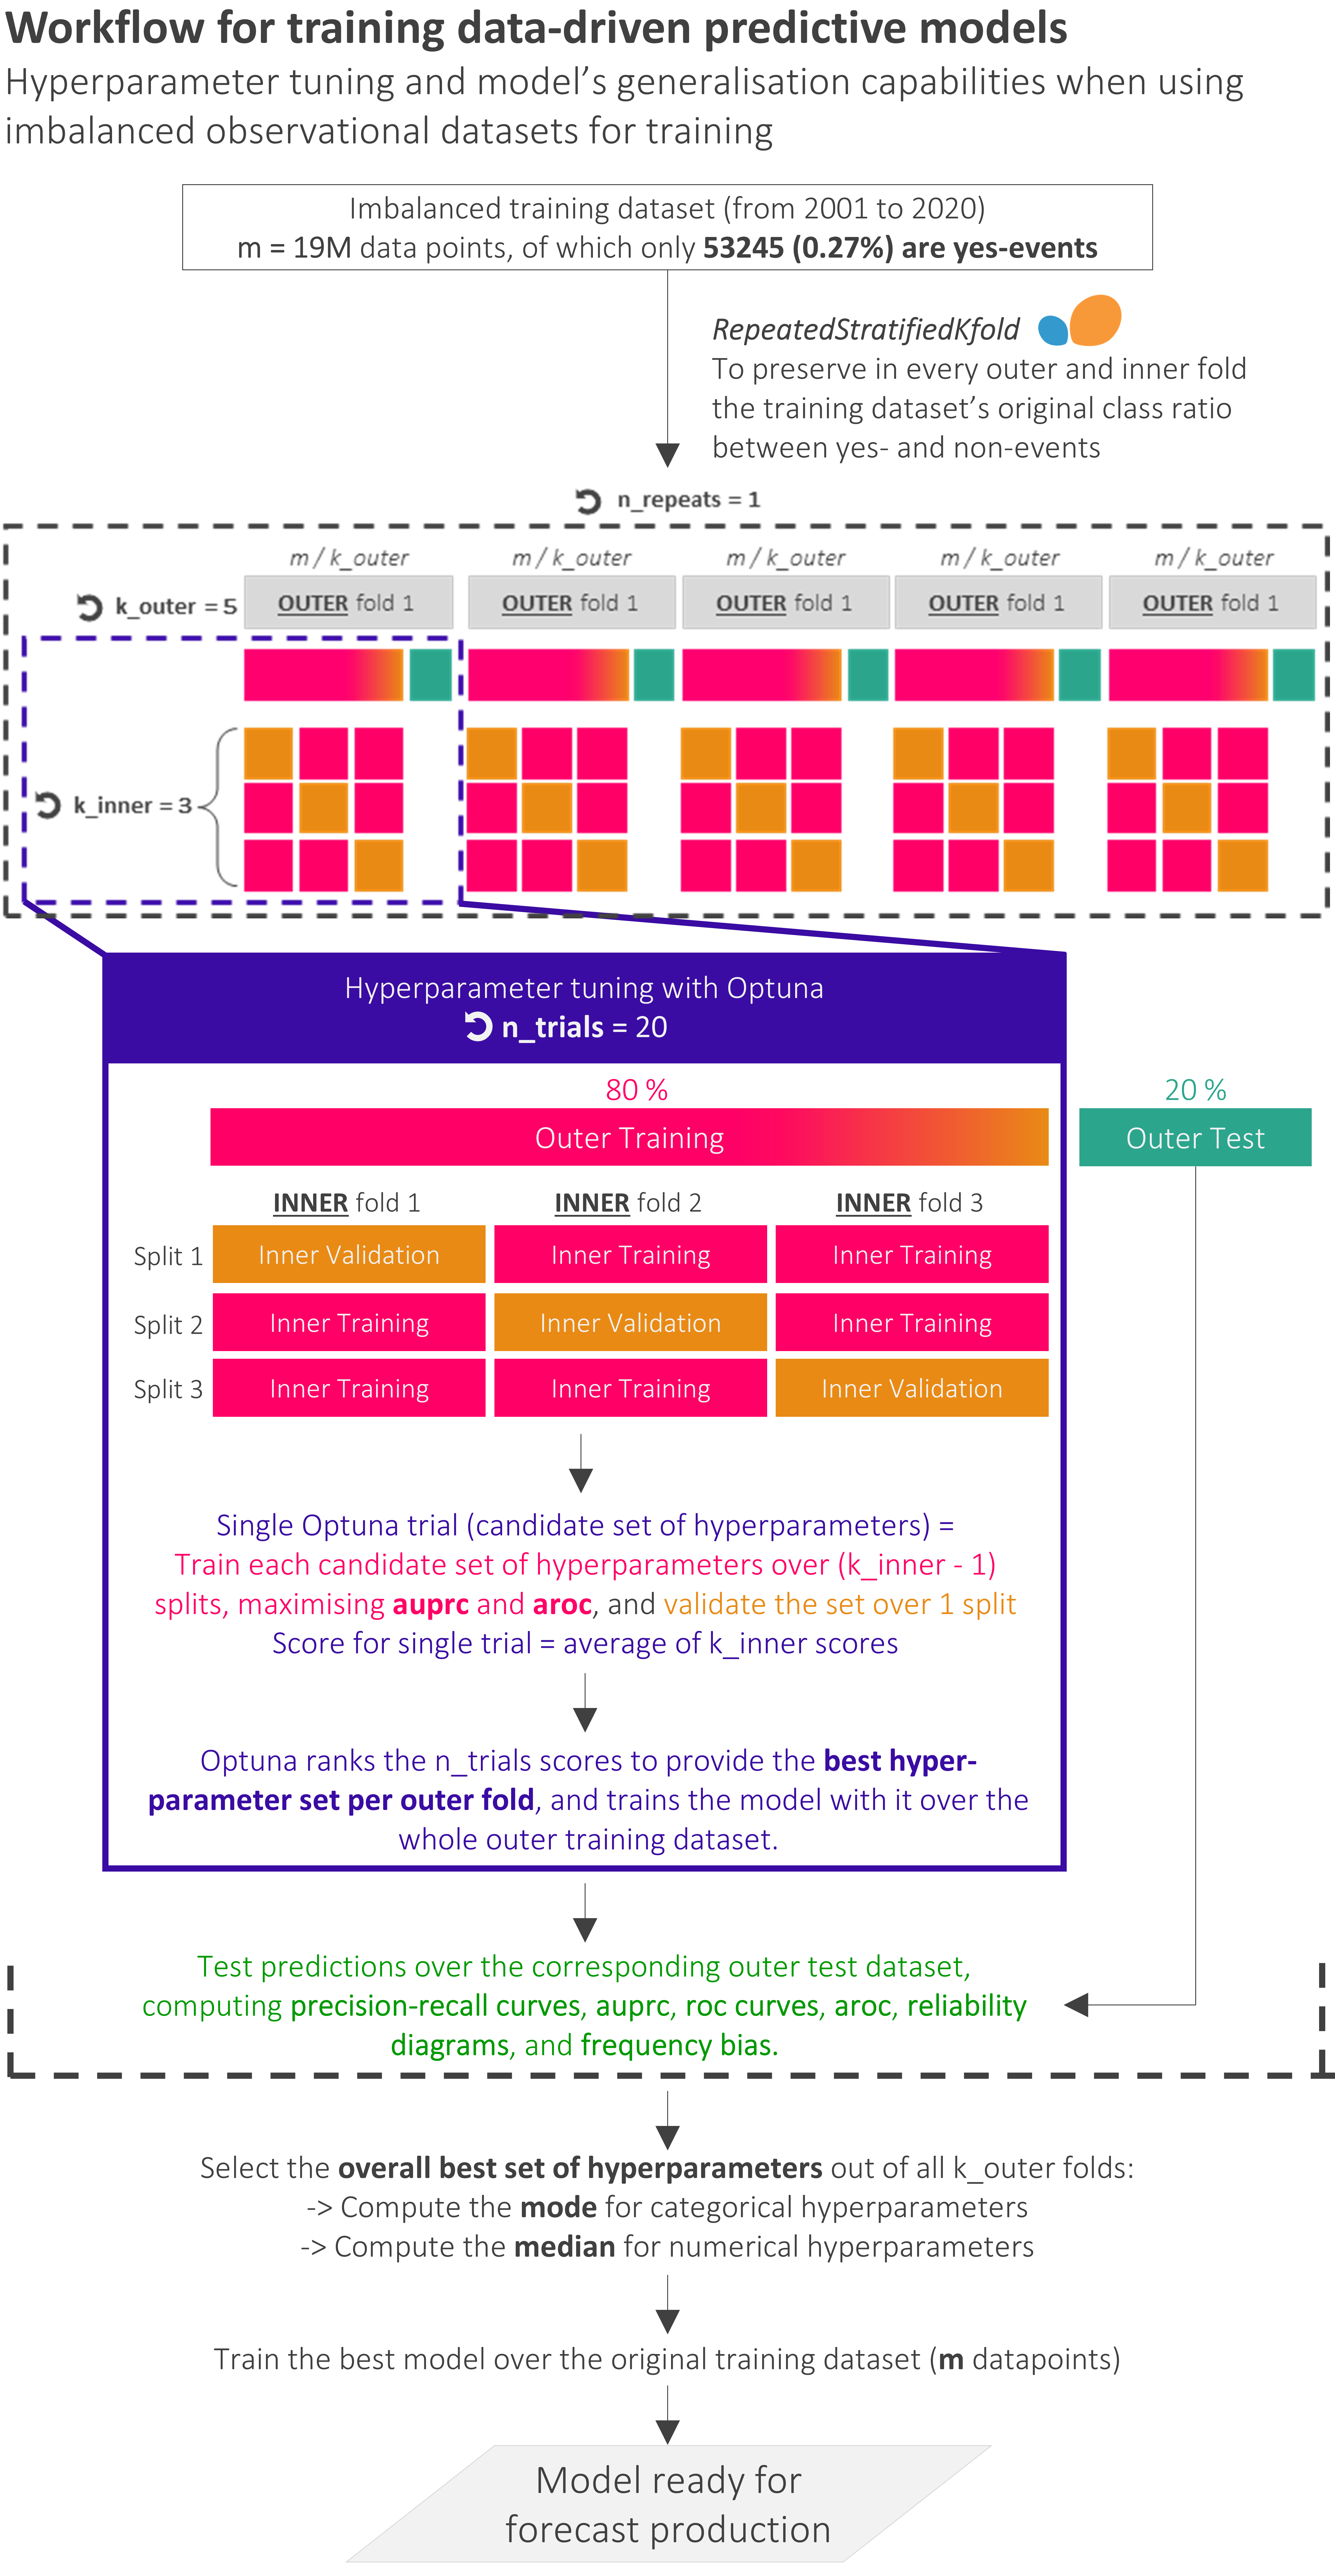
\includegraphics[scale = 0.95]{chapter_06/figures/cv_optuna.png}
\caption{\textbf{Workflow for the repeated nested cross-validation.} The outer cross-validation loop utilises Scikit-Learn's "RepeatedStratifiedKFold" function to create k\_outer = 5 outer folds (grey blocks) across n\_repeats = 1 iterations. Each \textcolor{colourOuterFolds}{\textit{outer fold}} maintains the class distribution of the \textcolor{colourTraining}{\textit{training dataset}}, and it is split into an outer training dataset (80\%, blocks in shades of pink and orange) and an \textcolor{colourOuterTest}{\textit{outer test dataset}} (20\%). Within each outer fold, a Bayesian hyperparameter tuning is performed employing the Optuna library through an inner cross-validation procedure over n\_trial = 20 repetitions. Each trial evaluates candidate hyperparameters by training on \textcolor{colourInnerTraining}{\textit{inner training folds}} and validating on \textcolor{colourInnerValidation}{\textit{inner validation folds}}, with performance measured as the mean AUC-ROC or AUC-PR. The optimal hyperparameter set, identified by maximising the selected evaluation metric, is used to train the final model on the complete outer training subset. Model performance is assessed on the held-out \textcolor{colourOuterTest}{\textit{outer test fold}} using AUC-ROC and AUC-PR. The best-performing fold is retrained on the original \textcolor{colourTraining}{\textit{training dataset}} for operational deployment. Independent, more extensive verification of the data-driven predictions is performed using the \textcolor{colourTest}{\textit{verification dataset}}, considering the Precision-Recall curve and AUC-PR, the ROC curve and AUC-ROC, reliability diagrams, and frequency bias.}
\label{fig:cv_optuna}
\end{figure}


\subsection{Hyperparameter tuning}

The \marginpara{Hyperparameter tuning: Optuna implementation} hyperparameter tuning was conducted using the Python library Optuna \citep{Akiba_2019}. The framework implements a Bayesian optimisation algorithm, primarily utilising the Tree-structured Parzen Estimator (TPE) sampler, which models the relationship between hyperparameters and objective function values to navigate high-dimensional search spaces efficiently. This approach significantly outperforms traditional grid search and random search methods, particularly when computational resources are limited or when the hyperparameter space is complex and continuous. The framework's architecture enables dynamic construction of search spaces where hyperparameters can be conditionally dependent on one another. Optuna's pruning capabilities represent a crucial innovation for computationally intensive tasks, allowing early termination of unpromising trials based on intermediate performance metrics. Moreover, the MedianPruner implementations monitor trial progress and eliminate configurations that are statistically unlikely to surpass previously observed performance, thereby focusing computational resources on promising regions of the hyperparameter space. This feature proves particularly valuable when training deep neural networks or large ensemble models, where individual trial evaluation may require substantial time. Optuna's integration with popular machine learning frameworks such as XGBoost, LightGBM, CatBoost, and TensorFlow handle framework-specific optimisations such as early stopping criteria and validation monitoring, whilst maintaining compatibility with Optuna's pruning mechanisms. Finally, the comprehensive logging and visualisation capabilities facilitate post-hoc analysis of optimisation trajectories, parameter importance assessment, and convergence diagnostics, providing valuable insights into model behaviour and hyperparameter interactions.

The Bayesian optimisation process conducted through Optuna evaluated n\_trial = 20 distinct hyperparameter configurations, with each trial exploring different regions of the search space guided by the Tree-structured Parzen Estimator algorithm.


\subsection{Loss functions}

The training framework implements a dual-strategy approach to address class imbalance through loss function configuration, enabling empirical determination of whether class weighting improves predictive performance for the specific characteristics of flash flood data. 

For \marginpara{Standard loss functions for balanced datasets} balanced datasets or when class imbalance is not a primary concern, the standard \textit{binary cross-entropy (BCE) loss function} is employed without modification. The standard BCE treats the binary classes equally, computing the negative log-likelihood of the predicted probabilities without any weighting mechanism. For tree-based models, the equivalent implementations include \textit{binary:logistic} objective for XGBoost, \textit{binary} objective for LightGBM, and \textit{Logloss} objective for CatBoost. These standard formulations assume that misclassification costs are symmetric between classes and that the training data adequately represents the true class distribution, making them suitable when positive and negative instances occur with comparable frequency.

Due \marginpara{Specialised loss functions for imbalanced datasets} to the severe class imbalance inherent in the problem considered in this thesis, the \textit{weighted binary cross-entropy (W-BCE) loss function} is also considered. It assigns differential importance to minority class instances through an optimisable positive class weight parameter (i.e., the class weights are themselves a hyperparameter optimised with Optuna), within the range [1.0, 10.0]. This weighting mechanism compensates for the scarcity of positive examples by increasing their contribution to the overall loss calculation, thereby preventing the model from converging to a trivial solution that simply predicts the majority class, i.e., it penalises misclassifications of rare flash flood events more heavily than false positives. The implementation manifests differently across frameworks: XGBoost and LightGBM utilise the \textit{scale\_pos\_weight} parameter to directly multiply the loss contribution of positive instances, whilst CatBoost employs the \textit{CrossEntropy loss function} with inherent class weighting capabilities. For neural networks, the Keras implementation applies \textit{class weights during batch gradient computation}, effectively rebalancing the optimisation landscape to ensure adequate representation of rare events.


\subsection{Verification scores}
%To be completed. Similar to that one in Chapter 5. 



%%%%%%%%%%%%%%%%%
\section{Results}
\label{data_driven_flash_floods_short_medium_range_results}

\subsection{Model training}

\subsubsection{Hyperparameter optimisation}

The hyperparameter optimisation history plot (Figure \ref{fig:optuna_history}) shows the overall good performance of the Optuna library in identifying quickly (within the first 10 trial, orange lines) and with relatively small variations (grey lines) the sets of hyperparameters that maximise the chosen evaluation metrics (AUC-ROC and AUC-PR). Performance remains fairly consistent between different outer folds (lines in shades of grey and orange). The optimisation histories for AUC-ROC (Figure \ref{fig:optuna_history}a-l) and AUC-PR (Figure \ref{fig:optuna_history}m-x) are very similar, with plots for loss functions specific for imbalanced datasets (Figure \ref{fig:optuna_history}g-l and s-x) showing more variability, but in general better overall performance, than those for more general loss functions (Figure \ref{fig:optuna_history}a-f and m-r). 

\begin{figure}[htbp]
\centering
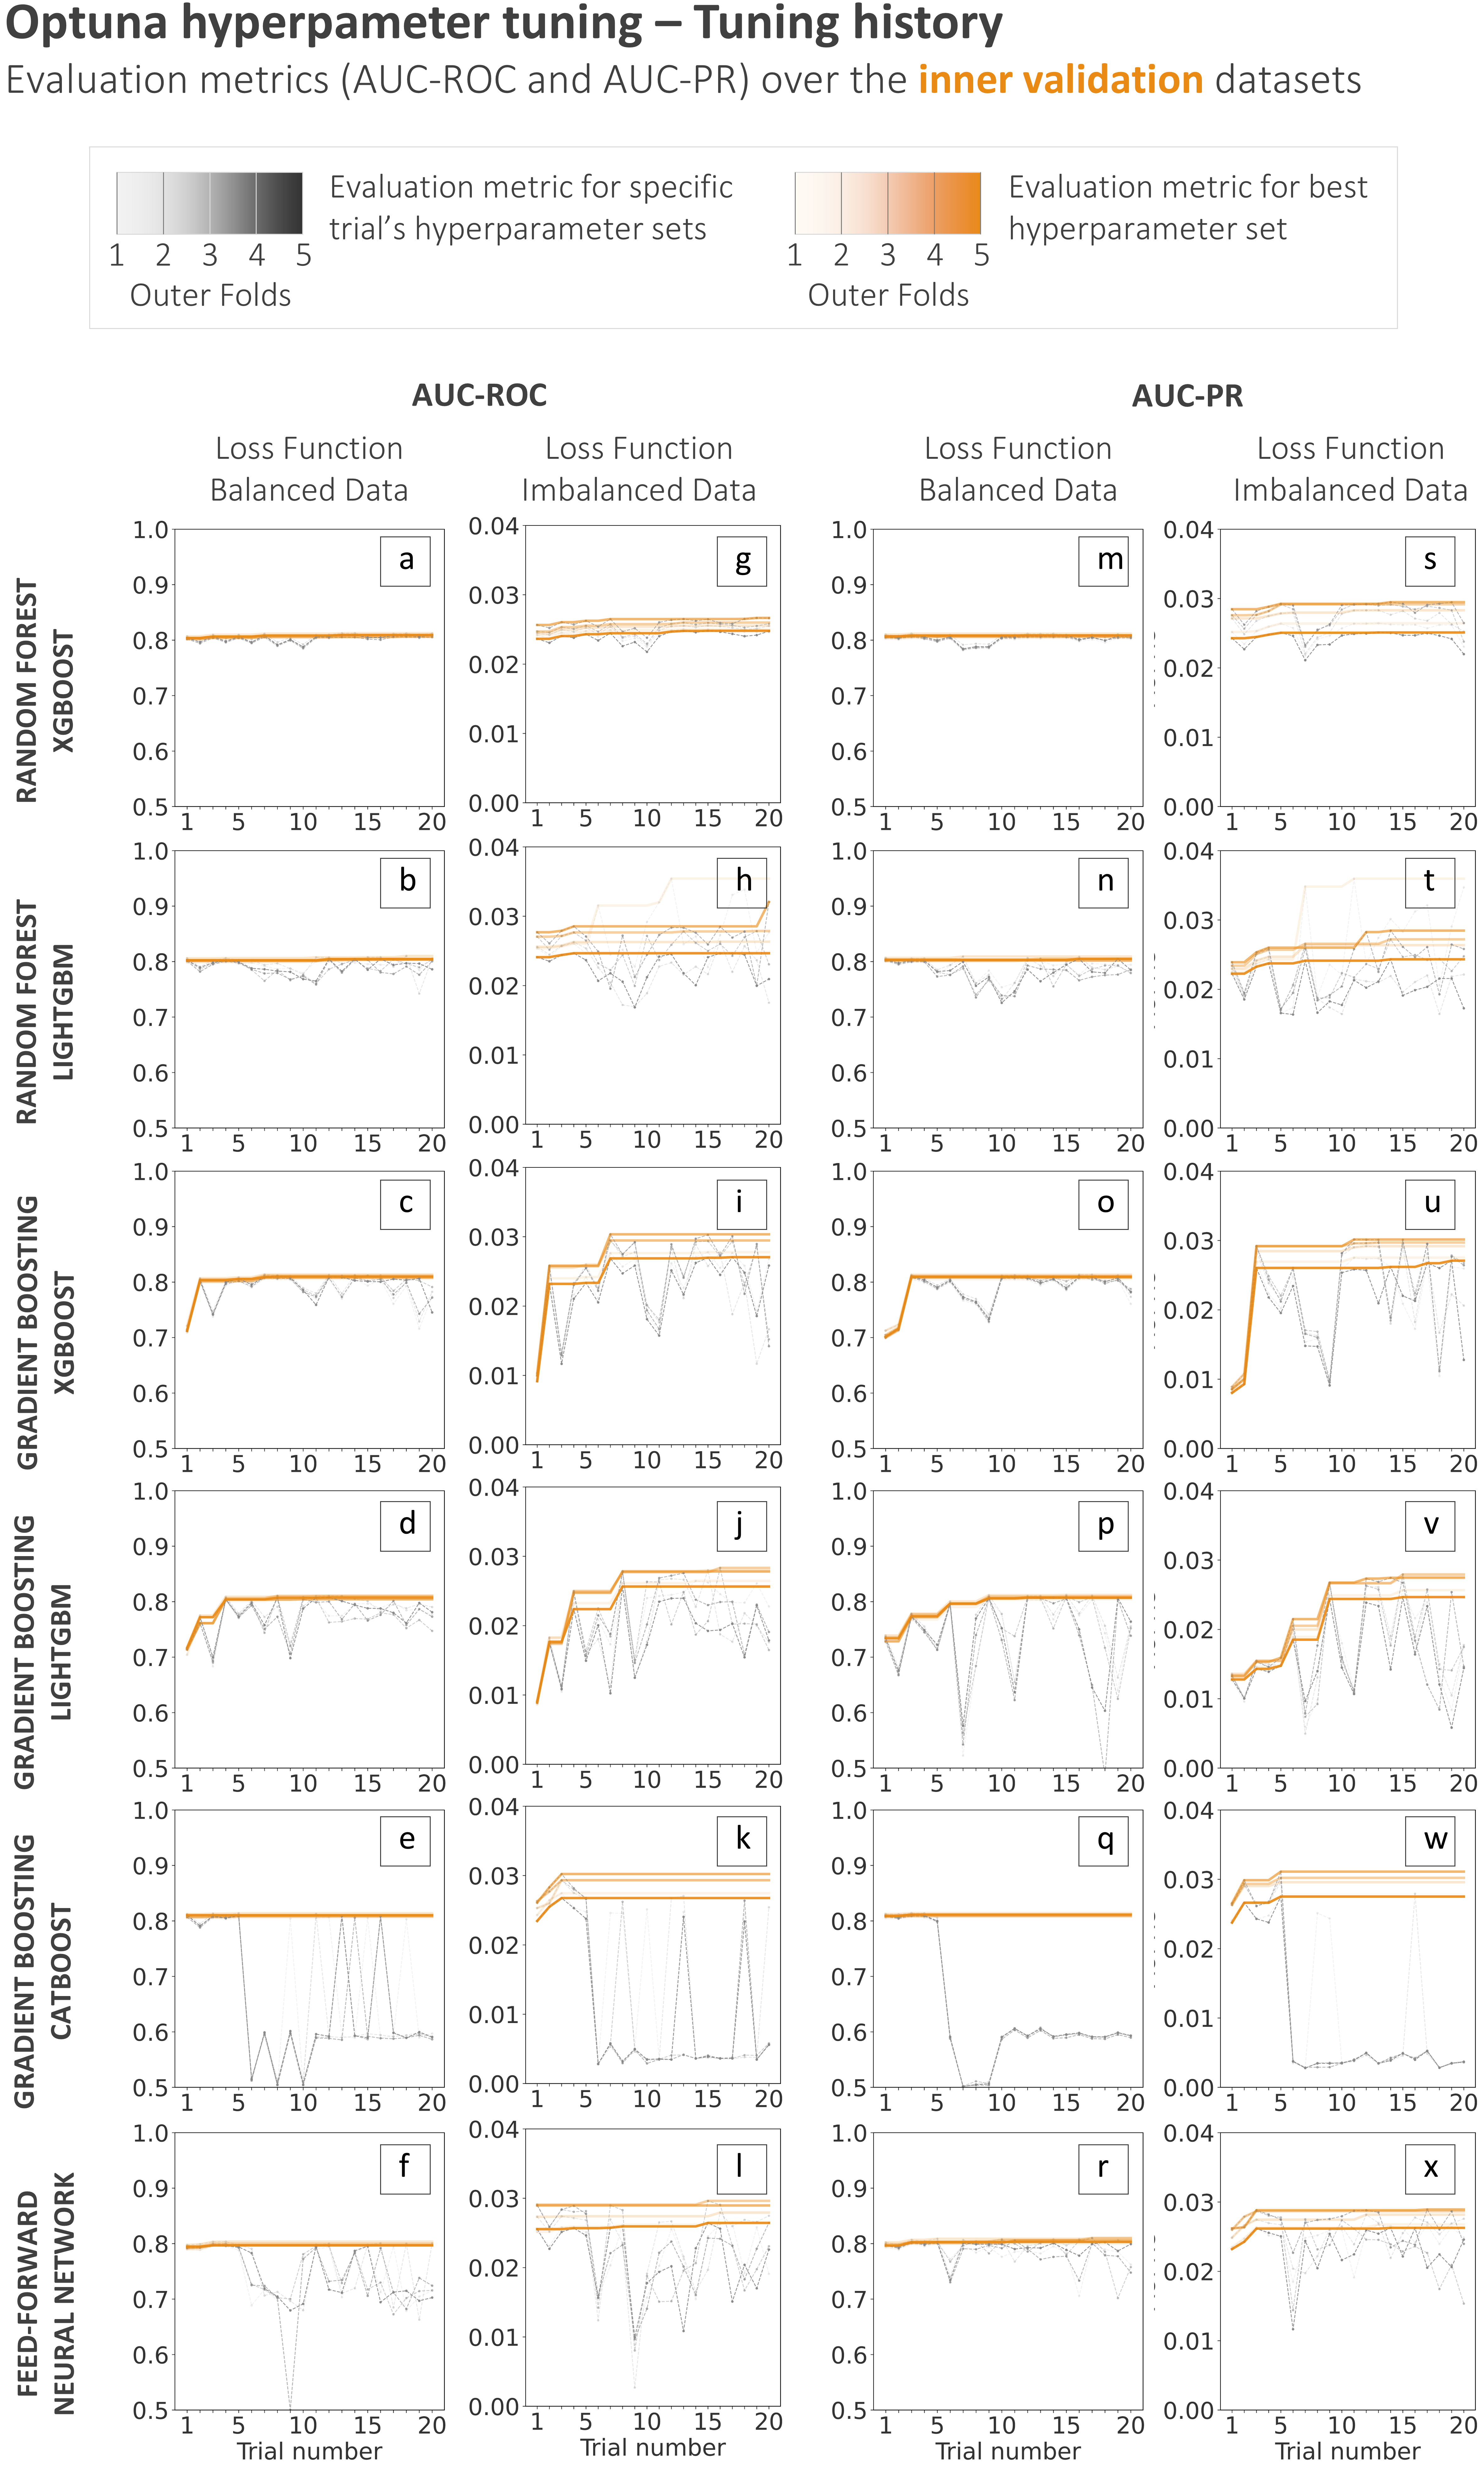
\includegraphics[width=\textwidth]{optuna_history.png}
\caption{\textbf{Optuna's hyperparameter optimisation history.} Evolution of the two evaluation metrics (AUC-ROC, panels (a) to (l) - and AUC-PR, panels (m) to (x)) maximised during the 20 trials run over the \textcolor{colourInnerTraining}{\textit{inner training folds}} to tune the hyperparameters of the six considered models (from top to bottom): random forest XGBoost, random forest LightGBM, gradient boosting XGBoost, gradient boosting LightGBM, gradient boosting CatBoost, and feed-forward neural network. The lines in shades of grey indicate individual trial performances, whilst lines in shades of orange highlight the best-performing hyperparameter set, identified by Optuna's Bayesian optimisation process. The shades of grey and orange represent the values of the evaluation metrics for each outer fold (lightest shade for the first outer fold and darkest for the latest). Panels (a) to (f) and (m) to (r) represents the results obtained using the standard binary cross-entropy loss functions - mostly used for balanced datasets - whilst panels (g) to (l) and (s) to (x) present the outcomes obtained with the weighted loss functions (specifically configured for imbalanced data).}
\label{fig:optuna_history}
\end{figure}

\subsubsection{Training progression and convergence}

Figure \ref{fig:hydro_based_ff_cross_validation_optuna_overall_scores} presents the performance stability across the five outer folds for all evaluated models for overall scores such as AROC, recall and F1-score. In all models, the AROC values exhibited remarkable consistency across folds, with the gradient boosting implementations (XGBoost and LightGBM) maintaining values between 0.84 and 0.86 throughout. The random forest variants demonstrated slightly lower (AROC between 0.81 and 0.83) but equally stable performance. The CatBoost implementation of gradient boosting showed the lowest performance (AROC \sim0.8) of all decision-tree-based models, and the feed-forward neural network showed the lowest performance with AROC values between 0.78 and 0.8. While XGBoost remains the best model based on the recall and the F1-score, the model ranking based on these metrics shows higher variability depending on the outer fold. The small variations in the scores' absolute values suggest that such ranking differences are primarily attributable to class imbalance sensitivity to rare positive instances rather than training instability. 

\begin{figure}[htbp]
\centering
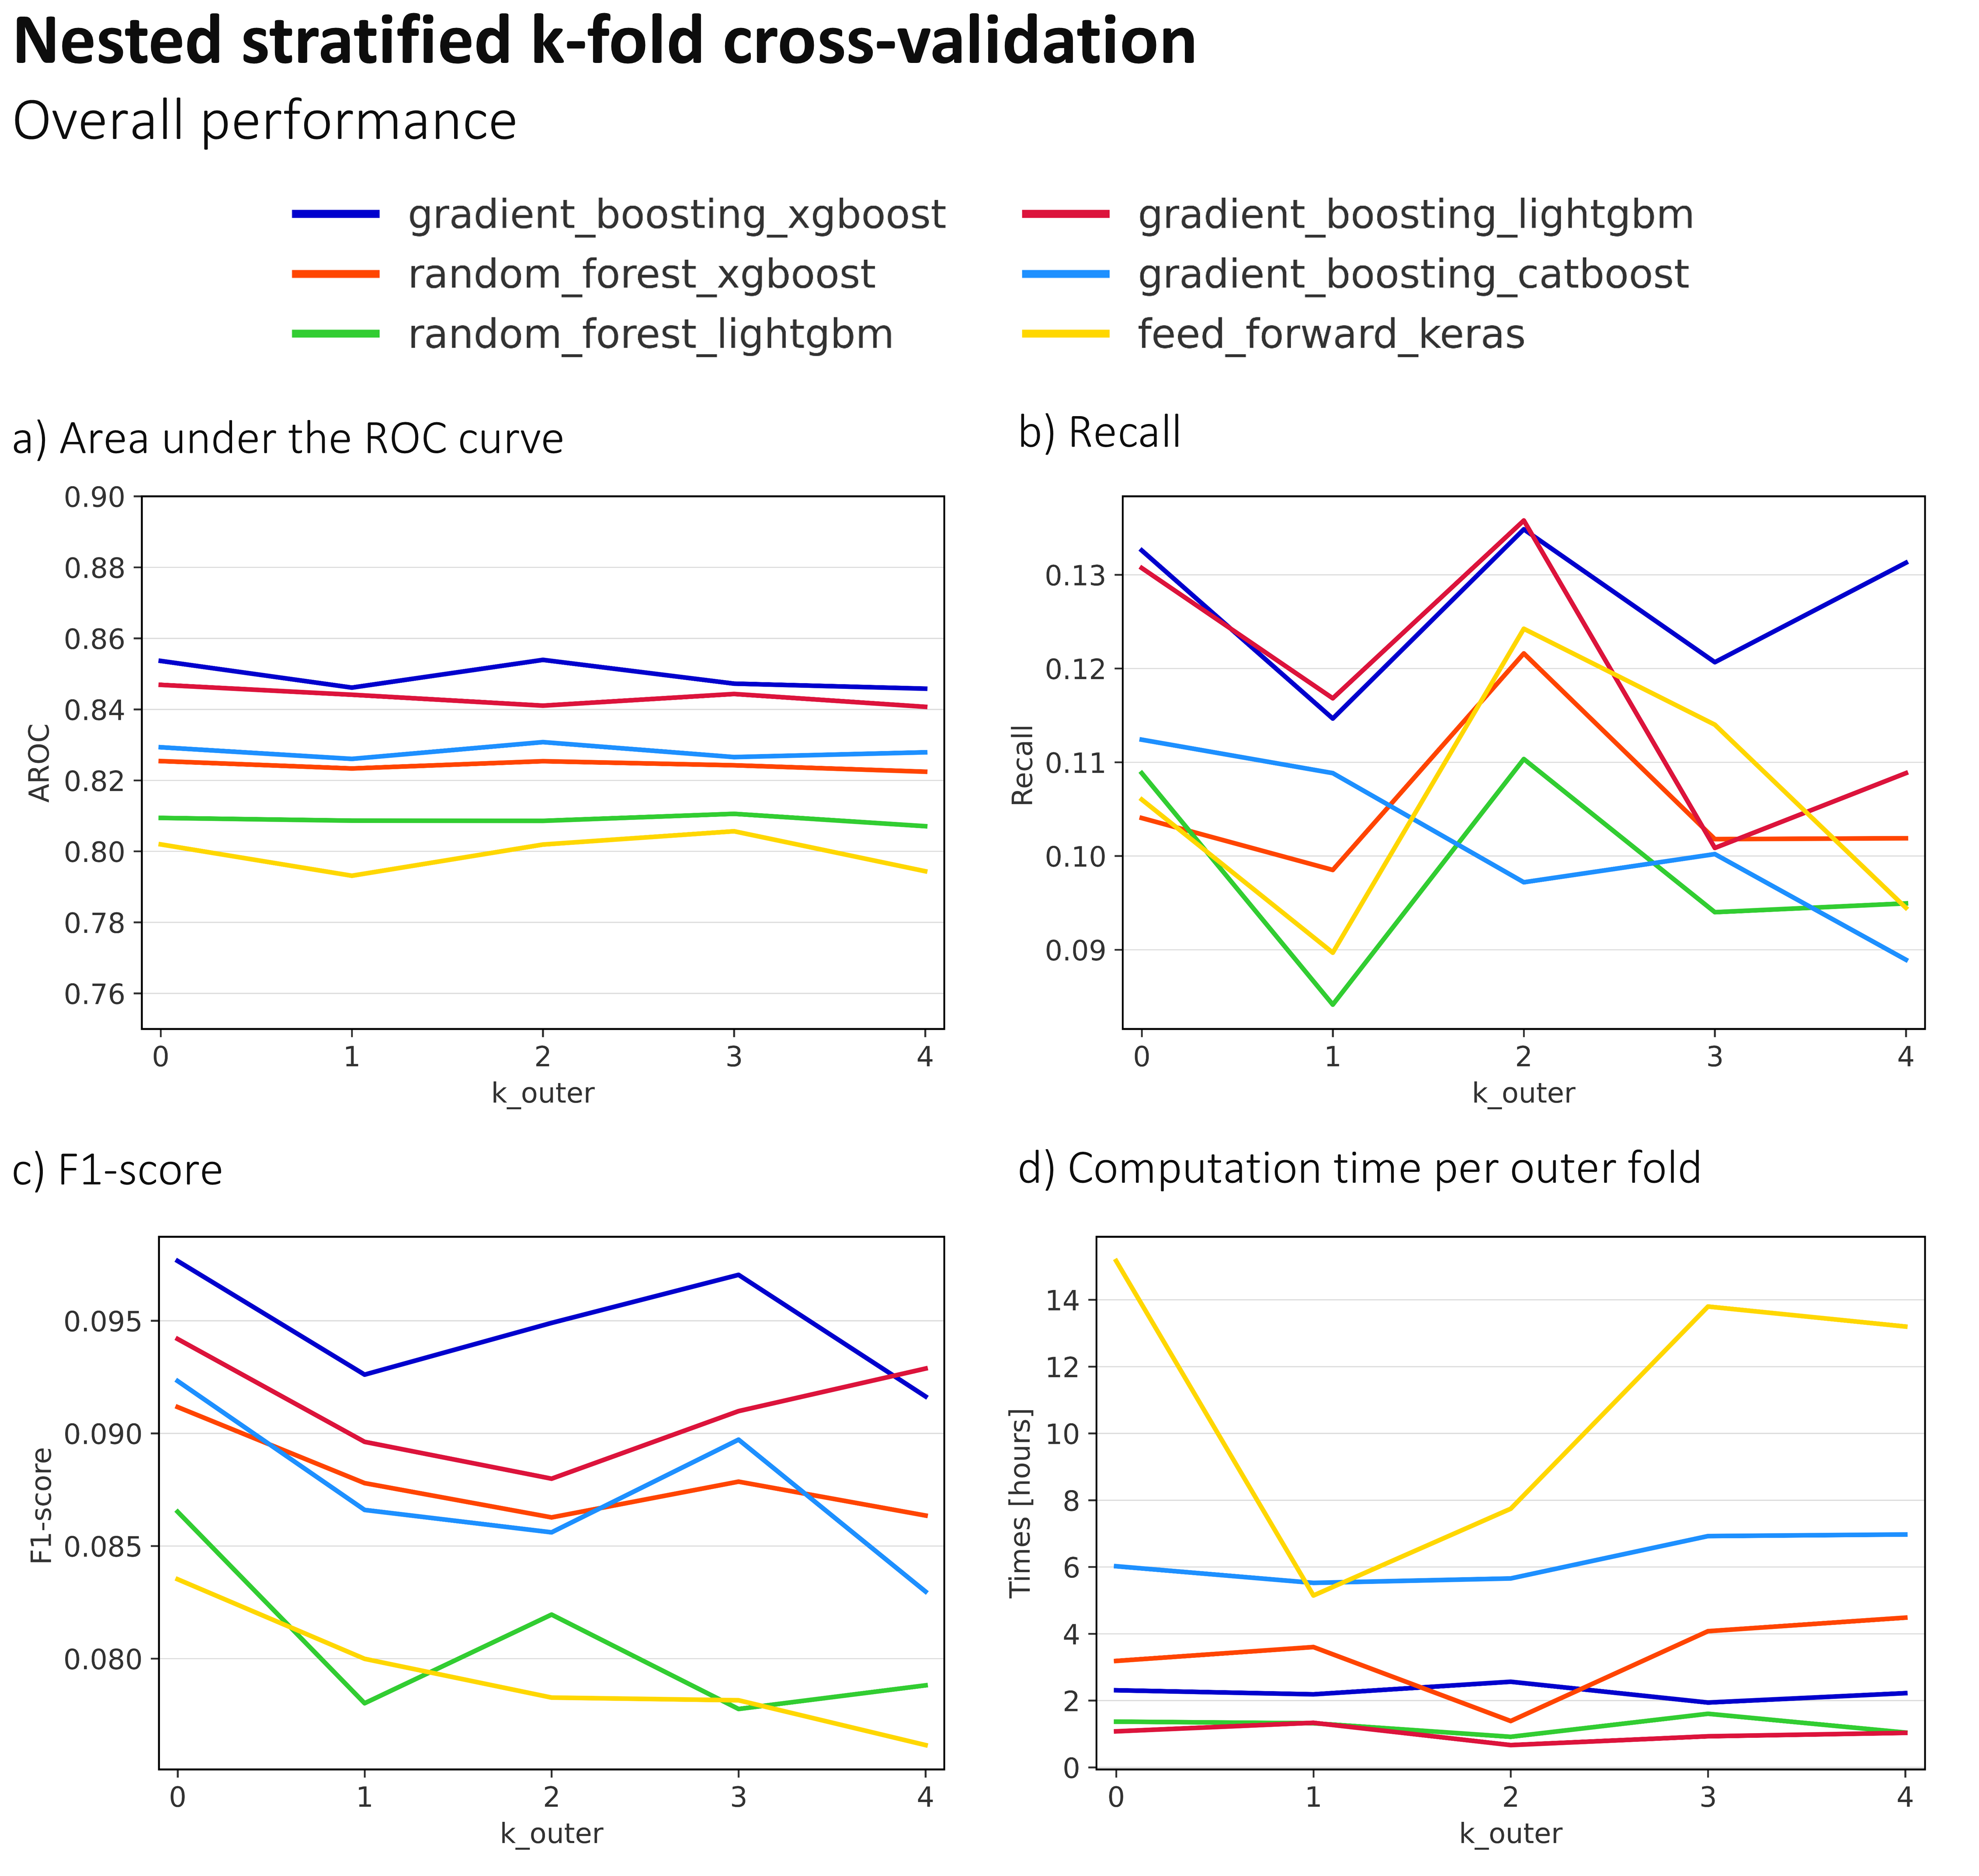
\includegraphics[width=\textwidth]{hydro_based_ff_cross_validation_optuna_overall_scores.png}
\caption{\textbf{Overall scores to estimate the model performance during the nested stratified k-fold cross validation.} Panels (a) to (d) show the values for, respectively, the area under the ROC curve, recall, F1-score, and training + hyperparameter optimisation time per outer fold. The solid colour lines represent the different models: gradient boosting - XGBoost implementation - in blue, gradient boosting - LightGBM implementation - in red, gradient boosting - CatBoost implementation - in cyan, random forest - XGBoost implementation - in orange, random forest - LightGBM implementation - in green, and feed forward neural network in yellow.}
\label{fig:hydro_based_ff_cross_validation_optuna_overall_scores}
\end{figure}

The ROC curves and the reliability diagrams (Figure \ref{fig:hydro_based_ff_cross_validation_optuna_breakdown_scores}) further illustrate the convergence quality by examining the discrimination ability and the reliability consistency across folds. Overall, the gradient boosting models (XGBoost - first column, LightGBM - second column, and Catboost - third column) show the best ROC curves and reliability diagrams, compared to the random forest implementations and the neural network, with high consistency across the outer folds. However, XGBoost shows again the best performance of all with the "optimal operating point" in the ROC curves being at a hit rate around \sim0.8 and a false alarm rate around only \sim0.3, and predicted probabilities in the reliability diagram closely aligning with the observed frequencies across most probability ranges (up to 25\% and reaching 50\% in the outer fold 1). While the other models show similar ROC curves, although with optimal operating points around hit rate of \sim0.7 for the decision-tree-based models and \sim0.6 for the neural network, the reliability diagrams for this models show a tendency to overestimate (i.e. the diagrams lie below the diagonal) from probabilities exceeding 10\% for the LightGBM and CatBoost implementations of the gradient boosting, and for almost all probability ranges in the random forest implementation of LightGBM. The XGBoost implementation of the random forest model shows a similar reliability to the XGBoost implementation of the gradient boosting, but the discrimination ability of the latter model is superior (better ROC curves over all outer folds). This suggests that \textit{gradient boosting} performs overall better than random forests when using imbalanced training datasets.

Special attention should be given to the neural network as it shows an overall good reliability (i.e. the predicted probabilities are close to the diagonal) but,  compared to the decision-tree-based models, the neural network does not provide high predicted probabilities, as they do not exceed 25\% (it reaches 50\% in only one outer fold). This behaviour suggests that the neural network demonstrates a conservative but reliable forecasting behaviour. While the neural network restraint in issuing high-probability forecasts might reflect a better uncertainty quantification and more reliable risk communication for operational deployment, the XGBoost implementation of the gradient boosting shows that predicted probabilities higher than 25\% can also be reliable between 30\% and 50\%. This restricted probability range in the neural network predictions presents operational challenges, as the model fails to differentiate between moderate and high-risk events, as shown by the lower discrimination ability of the neural network compared to XGBoost.. The inability to forecast probabilities above 25\% effectively compresses the decision space for emergency managers, who require clearer discrimination between events warranting different levels of response. Whilst a forecast of 25\% probability might trigger initial preparedness measures, operational protocols often stipulate enhanced response actions at higher probability thresholds (e.g., 40\%, 60\%). The neural network's truncated probability distribution therefore limits its utility in supporting graduated response strategies, potentially resulting in either insufficient preparation for genuinely high-risk events or uniform treatment of situations with materially different risk levels. This operational limitation suggests that, despite its superior calibration at lower probabilities, the neural network may be less suitable than the gradient boosting approaches for applications requiring nuanced risk stratification.

\begin{figure}[htbp]
\centering
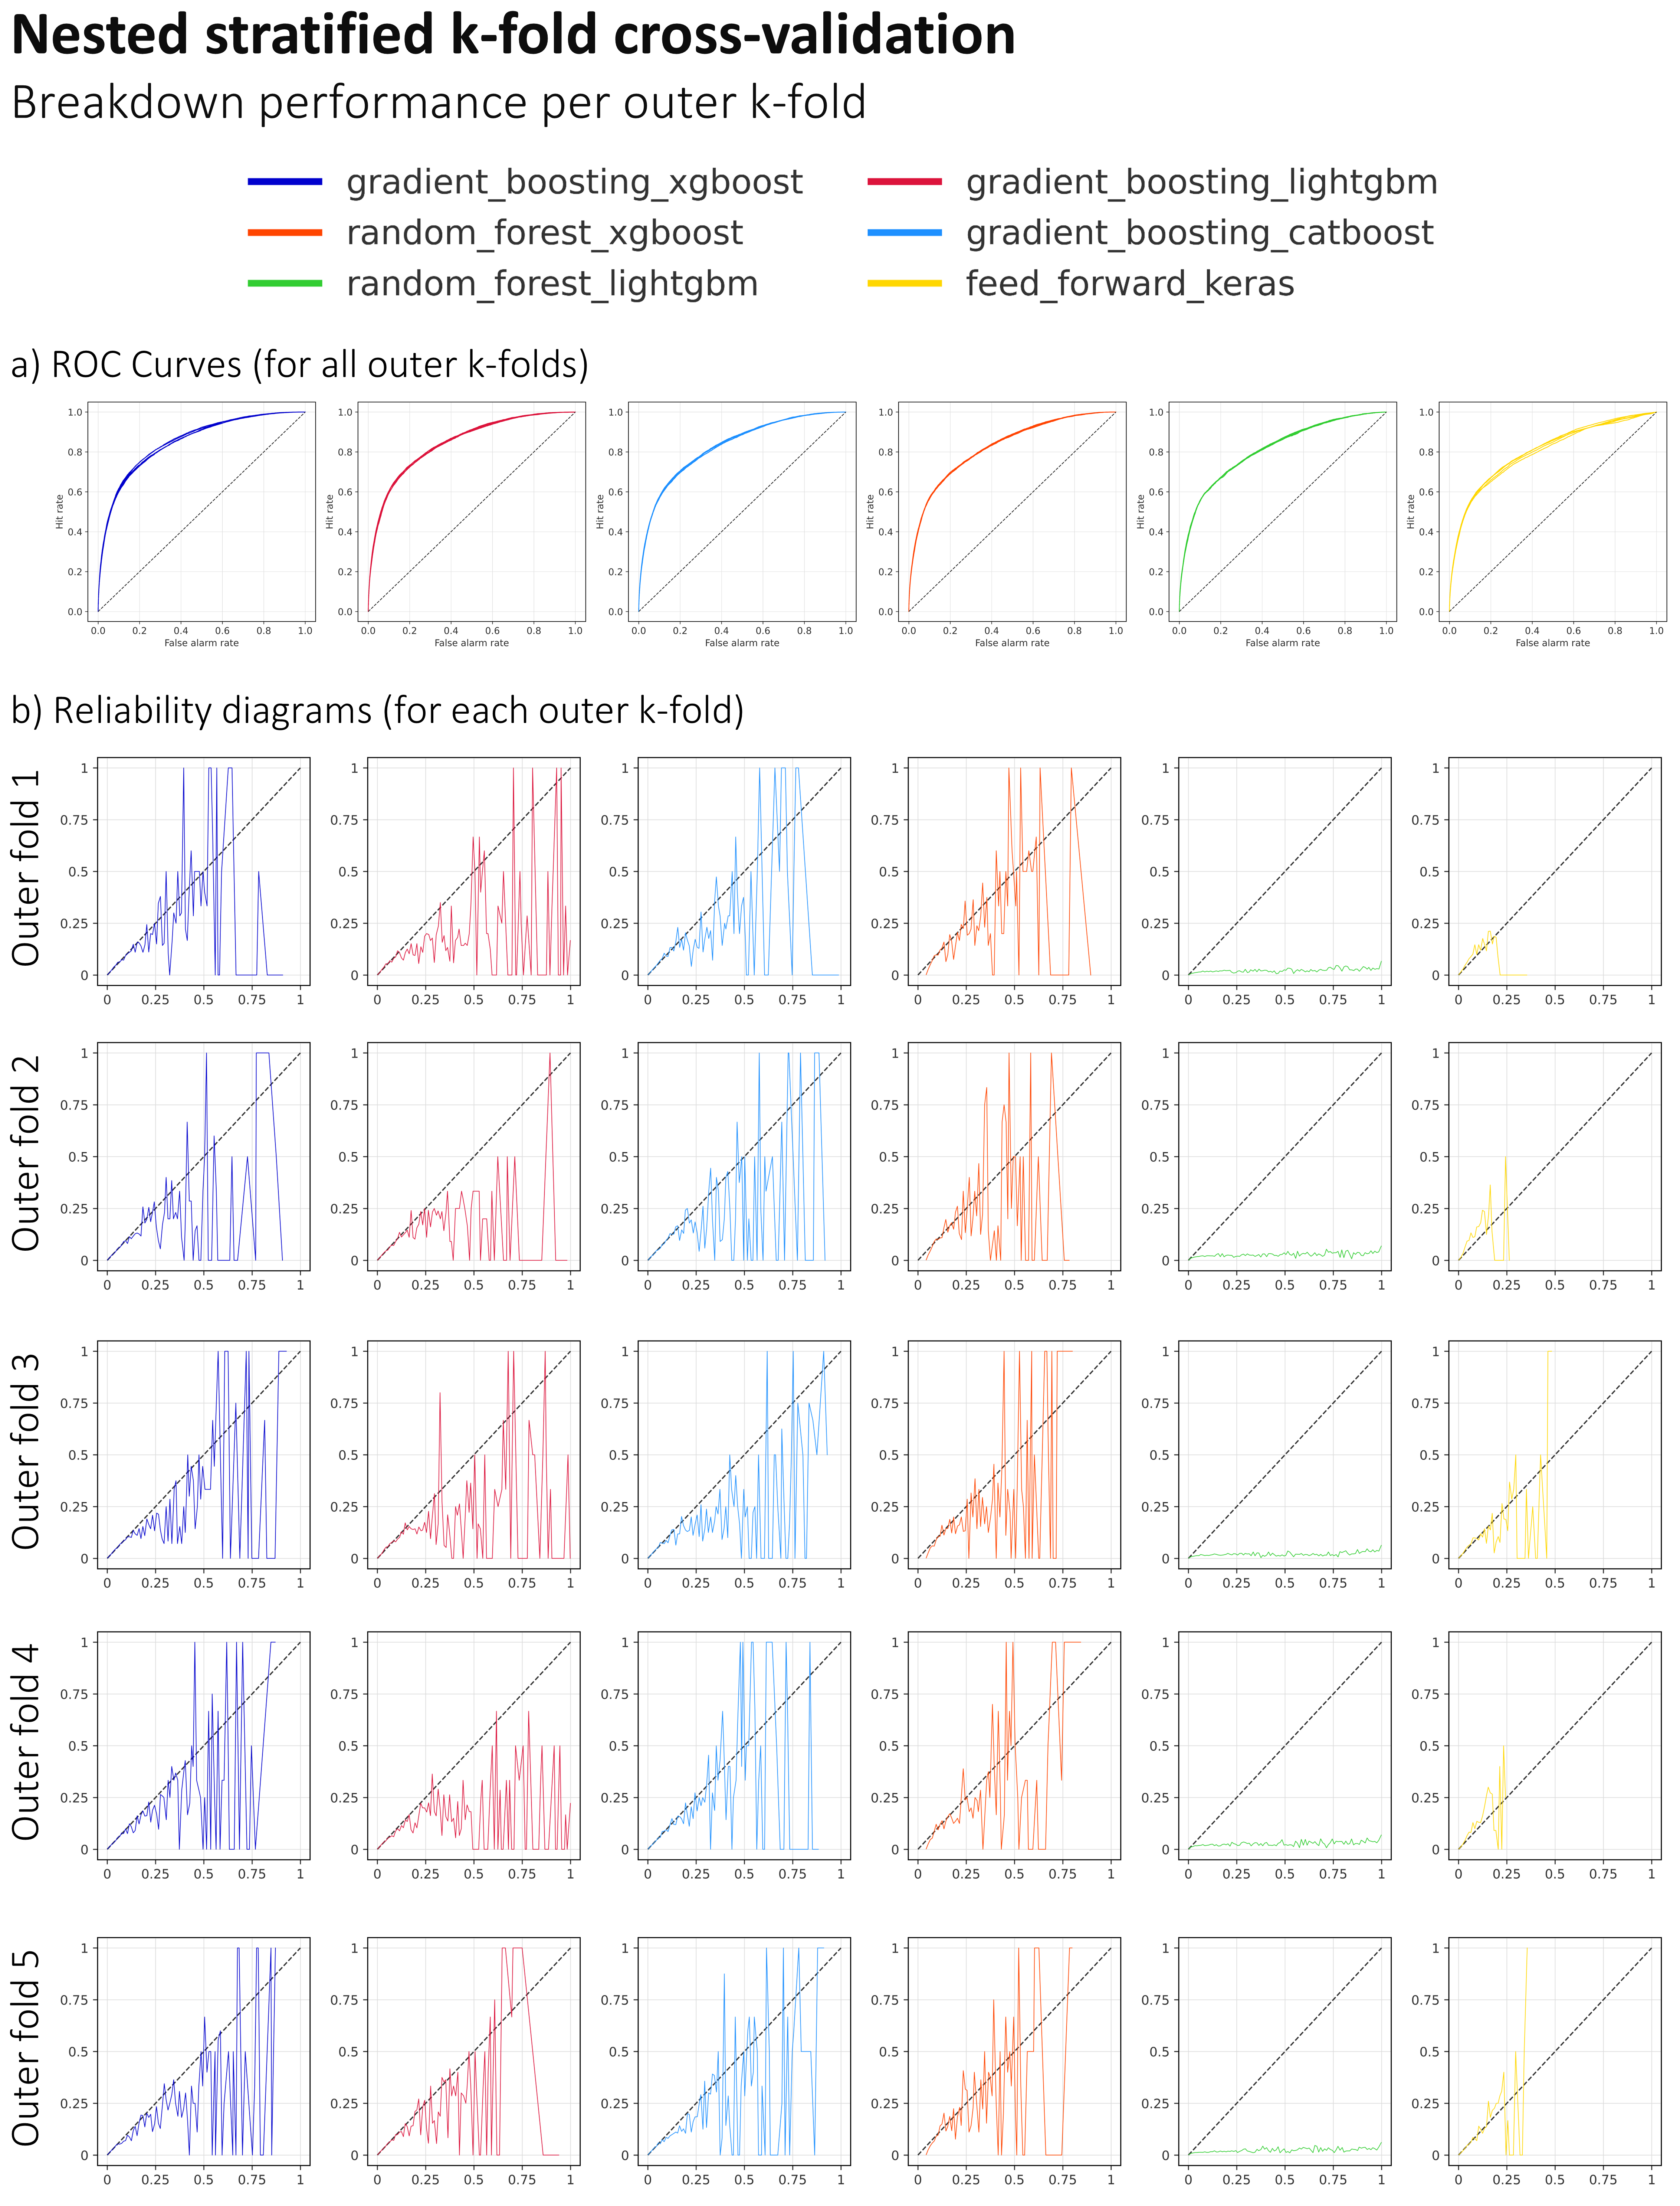
\includegraphics[width=\textwidth]{hydro_based_ff_cross_validation_optuna_breakdown_scores.png}
\caption{\textbf{Breakdown scores to estimate the model performance during the nested stratified k-fold cross validation.} Figures in panel (a) show the ROC curves for all the outer loops for gradient boosting - XGBoost implementation - in blue, gradient boosting - LightGBM implementation - in red, gradient boosting - CatBoost implementation - in cyan, random forest - XGBoost implementation - in orange, random forest - LightGBM implementation - in green, and feed forward neural network in yellow. Figures in panel (b) show the reliability diagrams for each outer loop (rows) and each model (columns).}
\label{fig:hydro_based_ff_cross_validation_optuna_breakdown_scores}
\end{figure}

In conclusion, the stability of model rankings across folds provided additional evidence of training convergence. The gradient boosting XGBoost consistently achieved the highest discrimination performance, followed closely by LightGBM, whilst the random forest implementations and neural networks occupied lower performance tiers. This consistent hierarchy across independent training runs confirms that the observed performance differences reflect genuine algorithmic characteristics rather than training artefacts or convergence failures.


\subsubsection{Final model selection}

Based on the performance metrics across all outer cross-validation folds (Figure \ref{fig:hydro_based_ff_cross_validation_optuna_overall_scores} and Figure \ref{fig:hydro_based_ff_cross_validation_optuna_breakdown_scores}, the model considered in this thesis to create the predictions of areas at risk of flash floods is the XGBoost implementation of the gradient boosting.

To establish the final model configuration for deployment (Table \ref{}), the hyperparameter values were aggregated across the outer folds using the \textit{median for continuous parameters} and the \textit{mode for categorical parameters}. This ensemble approach provided robustness against fold-specific peculiarities whilst maintaining near-optimal performance. 

\begin{table}[htbp]
\centering
\captionof{table}{\textbf{Final (optimal) configuration for the XGBoost implementation of the gradient boosting}. Values of the hyperparameters.}
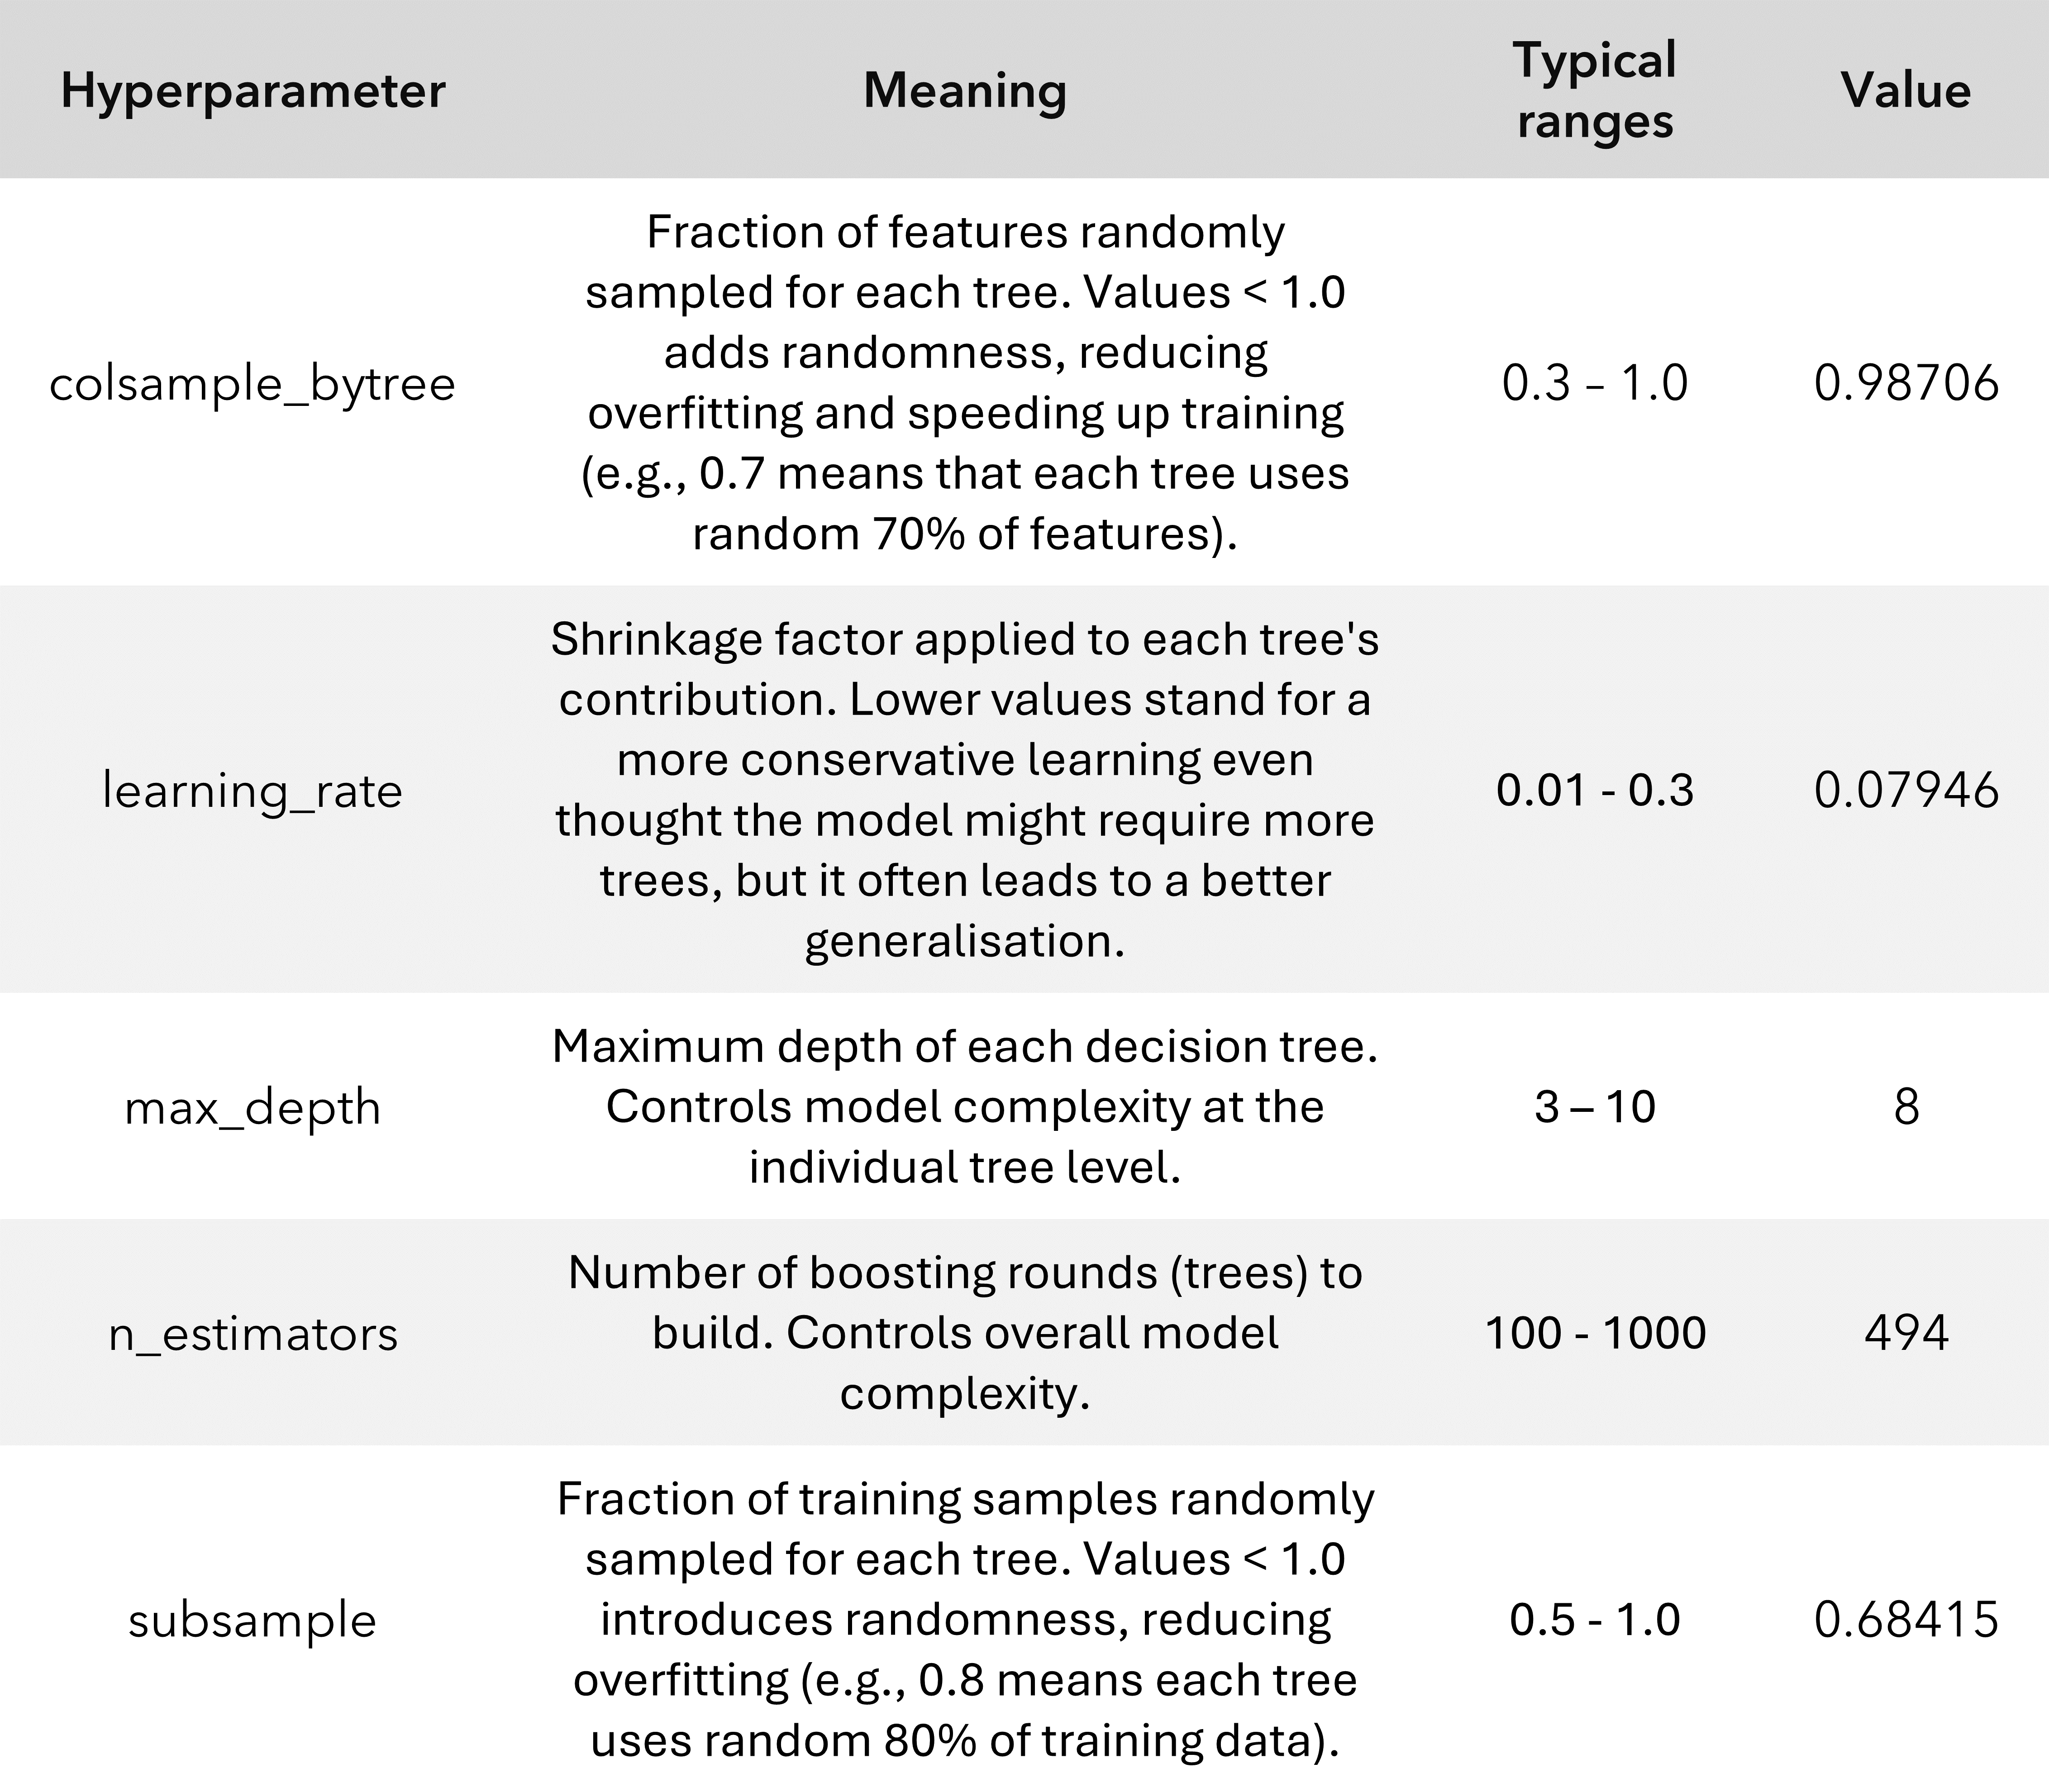
\includegraphics[width=\textwidth]{xgboost_final_configuration.png}
\label{table:xgboost_final_configuration}
\end{table}

The optimal XGBoost configuration identified through hyperparameter optimisation represents a moderately complex ensemble with careful regularisation to prevent overfitting. The model comprises 494 gradient boosted trees, each limited to a maximum depth of 8 levels, striking a balance between capturing non-linear patterns and maintaining interpretability. The learning rate of 0.07946 indicates a relatively conservative training approach, where each successive tree contributes only 7.9\% of its predictions to the ensemble, requiring the full complement of trees to achieve optimal performance whilst avoiding overshooting the loss function minima. This configuration employs substantial stochastic regularisation through both row and column subsampling: each tree is trained on a random 68.4\% of the training instances (subsample = 0.684) and utilises 98.7\% of available features (colsample\_bytree = 0.987). The high colsample\_bytree value (near 1.0) suggests that feature subsampling provides minimal regularisation benefit for this dataset, indicating that most predictors contribute meaningful information for flash flood prediction. Conversely, the moderate row subsampling (subsample = 0.68415) introduces beneficial stochasticity, helping the model generalise beyond the training data whilst maintaining sufficient data for reliable tree construction.

This configuration reflects a model that prioritises stability and generalisation over aggressive fitting, appropriate for the high-stakes nature of flash flood forecasting, where false alarms and missed events carry significant consequences. The parameter combination suggests the optimisation process favoured a large ensemble of moderately deep trees with conservative learning dynamics over a smaller set of more complex trees, likely improving the model's robustness to variations in hydro-meteorological conditions.

\subsubsection{Computation requirements}



\subsection{Assessment of short- and long-range data-driven hydro-meteorological predictions of areas at risk of flash floods}

\subsubsection{Overall verification scores}

Figure \ref{fig:hydro_based_ff_verif_overall_scores} presents the results of the objective verification analysis carried out on the hydro-meteorological, data-driven predictions of areas at risk of flash floods. It shows distinct performance characteristics between the short-range forecasts (also known as reanalysis) and the long-range forecasts (up to t +120, day 5). It is worth noticing that day 1 forecasts (t+24) have a very similar value compared to those for day 0 (short-range) forecasts, in all verification scores. 

The area under the ROC curve (Figure \ref{fig:hydro_based_ff_verif_overall_scores}a) shows forecasts with strong discrimination ability, maintaining values above 0.75 across all lead times. The short-range forecast (lead time 0) and day 1 forecasts achieve the highest discrimination performance with an AROC of approximately 0.83, indicating excellent ability to distinguish between flash flood and non-flash flood events. As lead time increases, the AROC exhibits a gradual linear decline, reaching \sim0.77 at day 5 forecasts (\sim7\% reduction in discrimination ability from day 0). Such a small reduction, especially compared to the rainfall-based forecasts, represents a modest degradation considering the extended forecast range, suggesting that the model maintains substantial predictive skill even at longer lead times.

The frequency bias (Figure \ref{fig:hydro_based_ff_verif_overall_scores}b) reveals a dramatic shift in forecast behaviour between short-range and long-range predictions. The day 1 forecasts show nearly identical frequency bias compared to day 0 (short-range) forecasts, i.e, \sim15. From day 2 forecasts, the frequency bias starts increasing, reaching a frequency bias that doubles the one at day 1 (\sim 31) at day 4. Comparing these results to the rainfall-based forecasts, where the frequency bias remains mostly constant over the different lead times, it would not be reasonable to think that the degradation of the frequency bias in the hydro-meteorological, data-driven forecasts are mainly due to variations in skill of the soil moisture with lead time, as the other parameters adopted in the data-driven model (orography and vegetation cover, are either static or climatological).

The recall (Figure \ref{fig:hydro_based_ff_verif_overall_scores}c) and F1-score (Figure \ref{fig:hydro_based_ff_verif_overall_scores}d) show a similar pattern. The day 1 forecasts show a slightly higher value compared to the one at day 0 (\sim 0.11 for recall and 0.08 for F1-score). From day 2, both scores half around day 5. This means that, according to both metrics, the model's ability to detect true positives deteriorates significantly beyond day 2, with the 5-day forecast detecting \sim half the events identified by the short-range forecast or the day 1 forecasts.

These verification metrics collectively indicate that the data-driven approach performs optimally at 0-1 day lead times, with acceptable performance extending to day 2. Beyond this threshold, whilst discrimination ability (AROC) remains reasonable, the operational utility diminishes substantially due to excessive false alarm rates and reduced detection capability, suggesting to further adjust the lead-time-dependent probability thresholds or alternative modelling strategies for extended-range flash flood forecasting.

\begin{figure}[htbp]
\centering
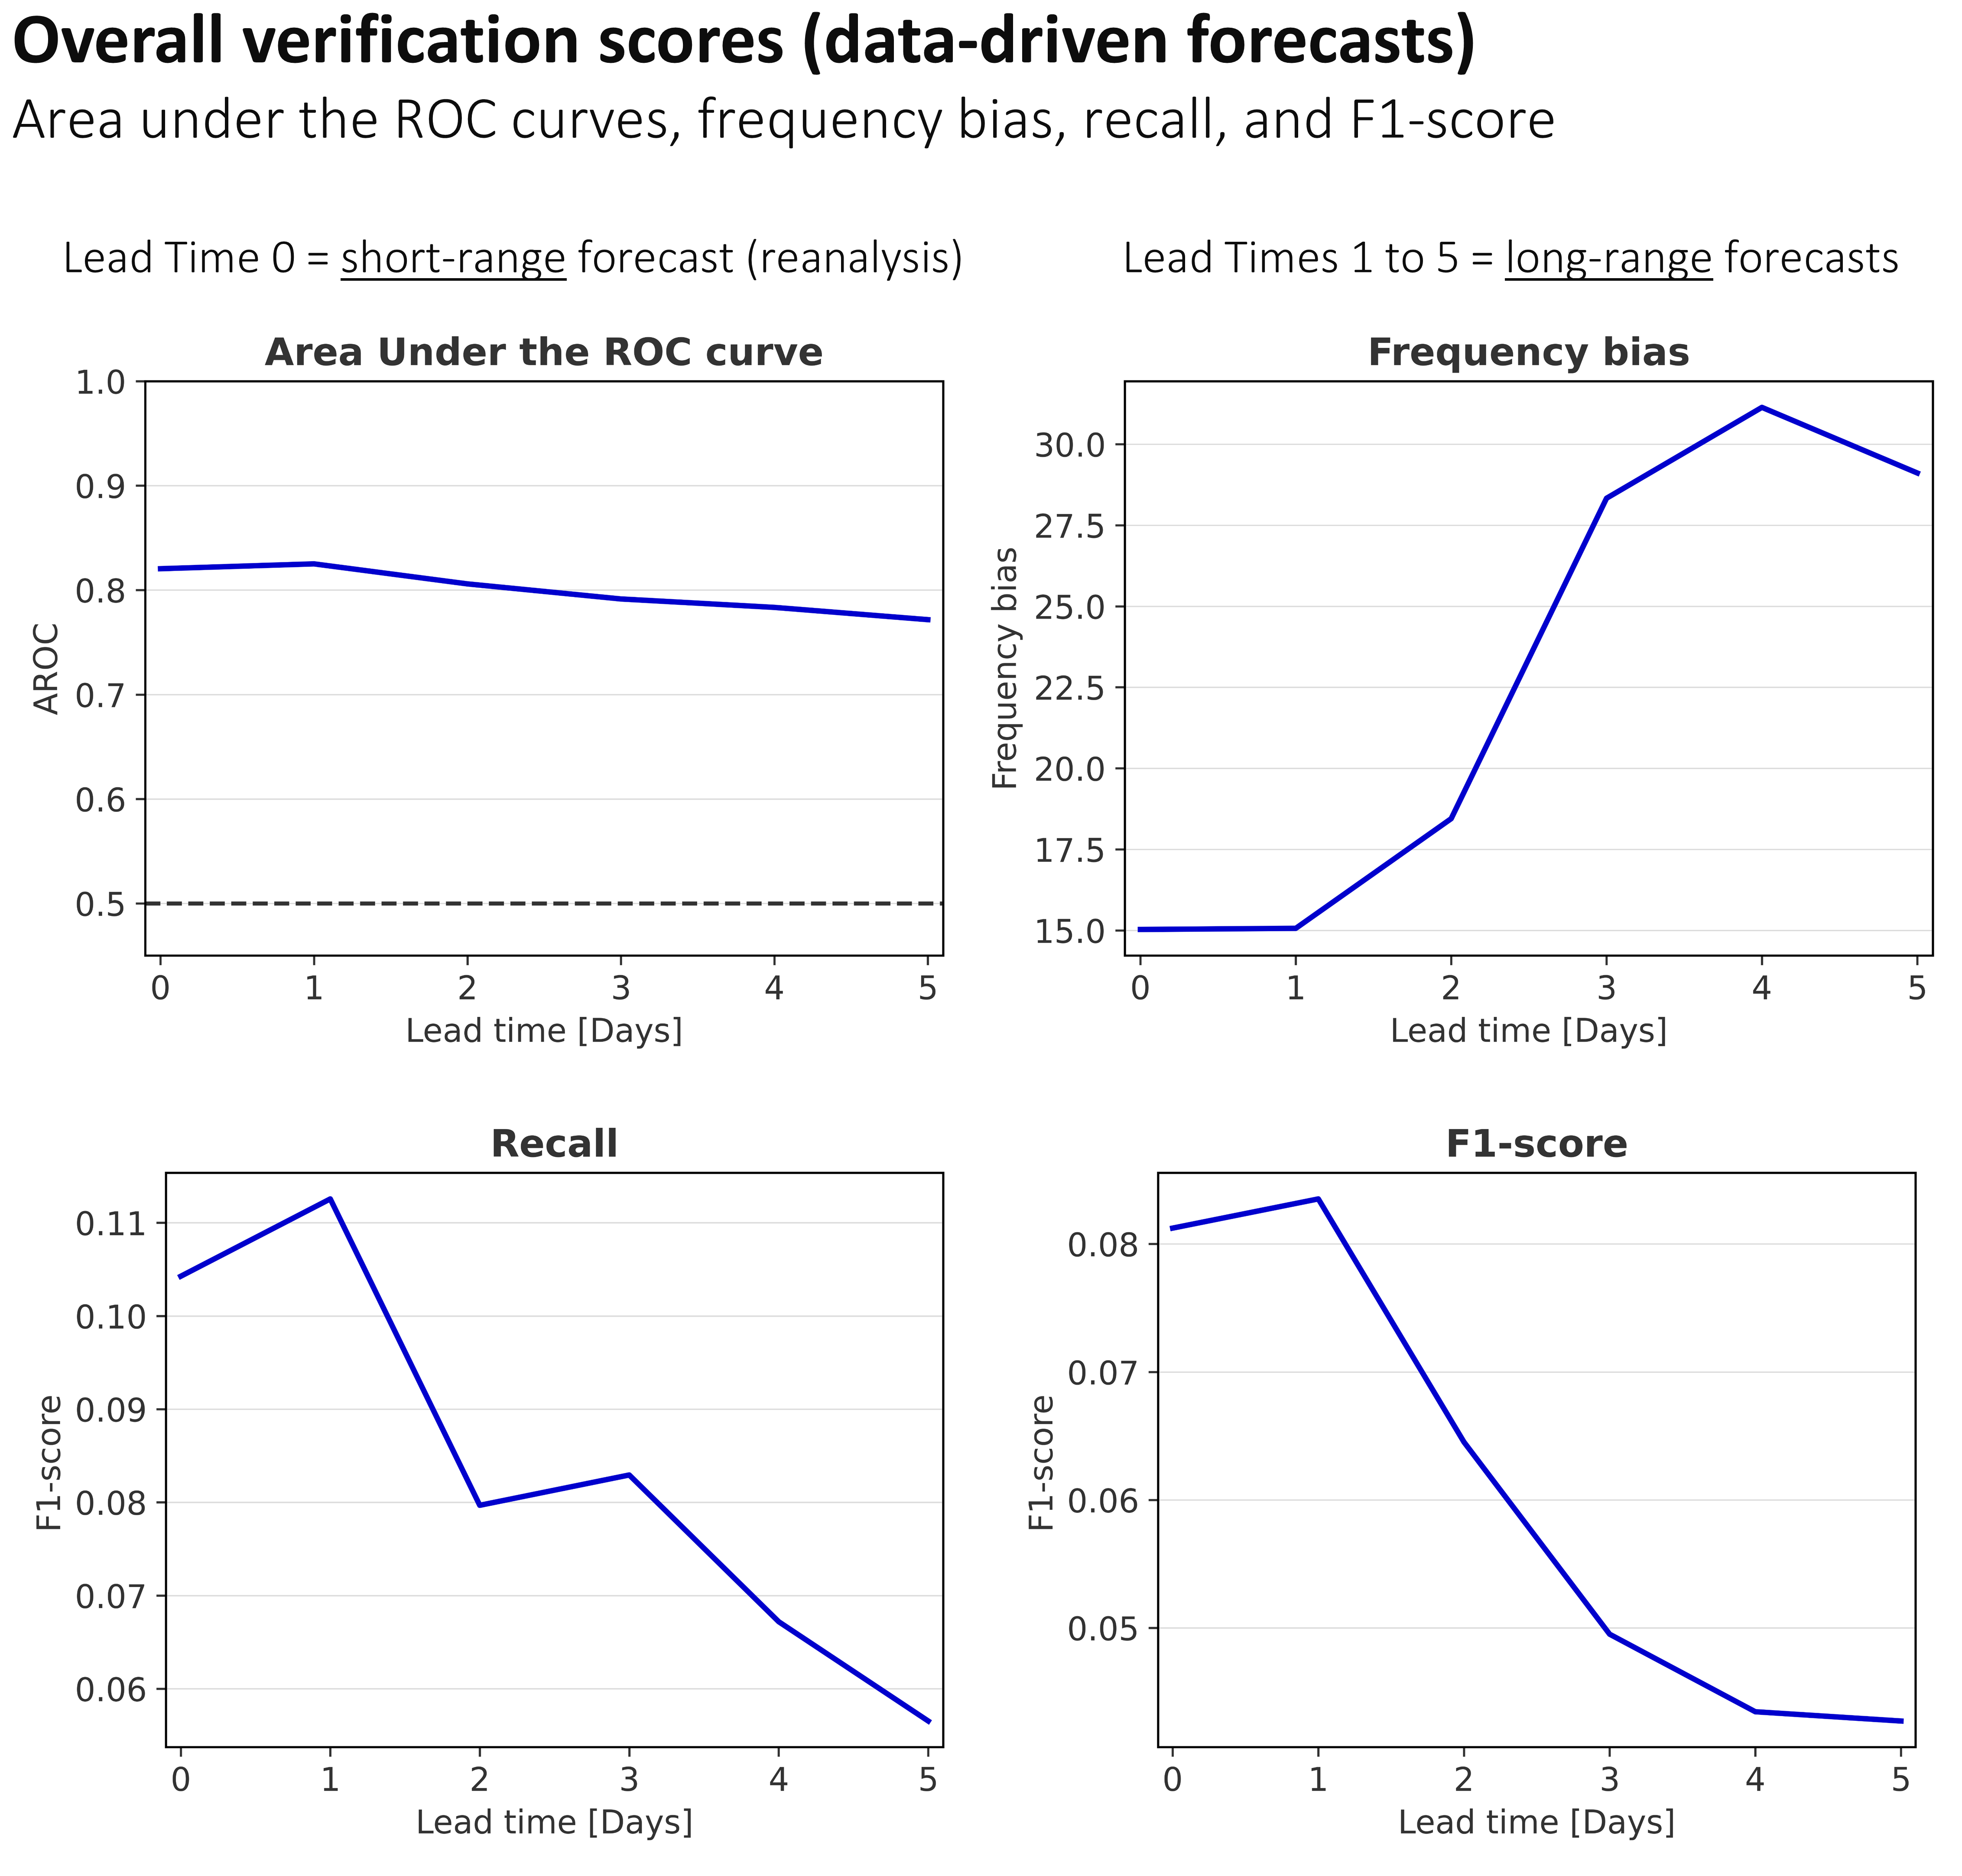
\includegraphics[width=\textwidth]{hydro_based_ff_verif_overall_scores.png}
\caption{\textbf{Overall verification scores for data-driven, hydro-meteorological forecasts.} Panel (a) shows the Area under the ROC curve for the short-range forecasts (i.e., reanalysis, lead time = 0), and the long-range forecasts (lead time = 1 - t+24, lead time = 2 - t+48, lead time = 3 - t+72, lead time = 4, t+96, lead time = 5, t+120). Panels (b) to (c) show, respectively, the frequency bias, the recall, and the F1-score.}
\label{fig:hydro_based_ff_verif_overall_scores}
\end{figure}

\subsubsection{Breakdown verification scores}

As seen in the overall verification scores, also the ROC curve for a day 1 (Figure \ref{fig:hydro_based_ff_verif_breakdown_scores_roc}, dashed line) forecast is nearly identical (almost perfect overlap) with day 0 forecasts (\ref{fig:hydro_based_ff_verif_breakdown_scores_roc}, solid and thicker line). Then, there is a small and gradual worsening of the ROC for longer-range forecasts observed by the flattening of the ROC curves towards the diagram's diagonal. Such flattening means that for a similar hit rate, the false alarms increase slightly, around 0.1.

\begin{figure}[htbp]
\centering
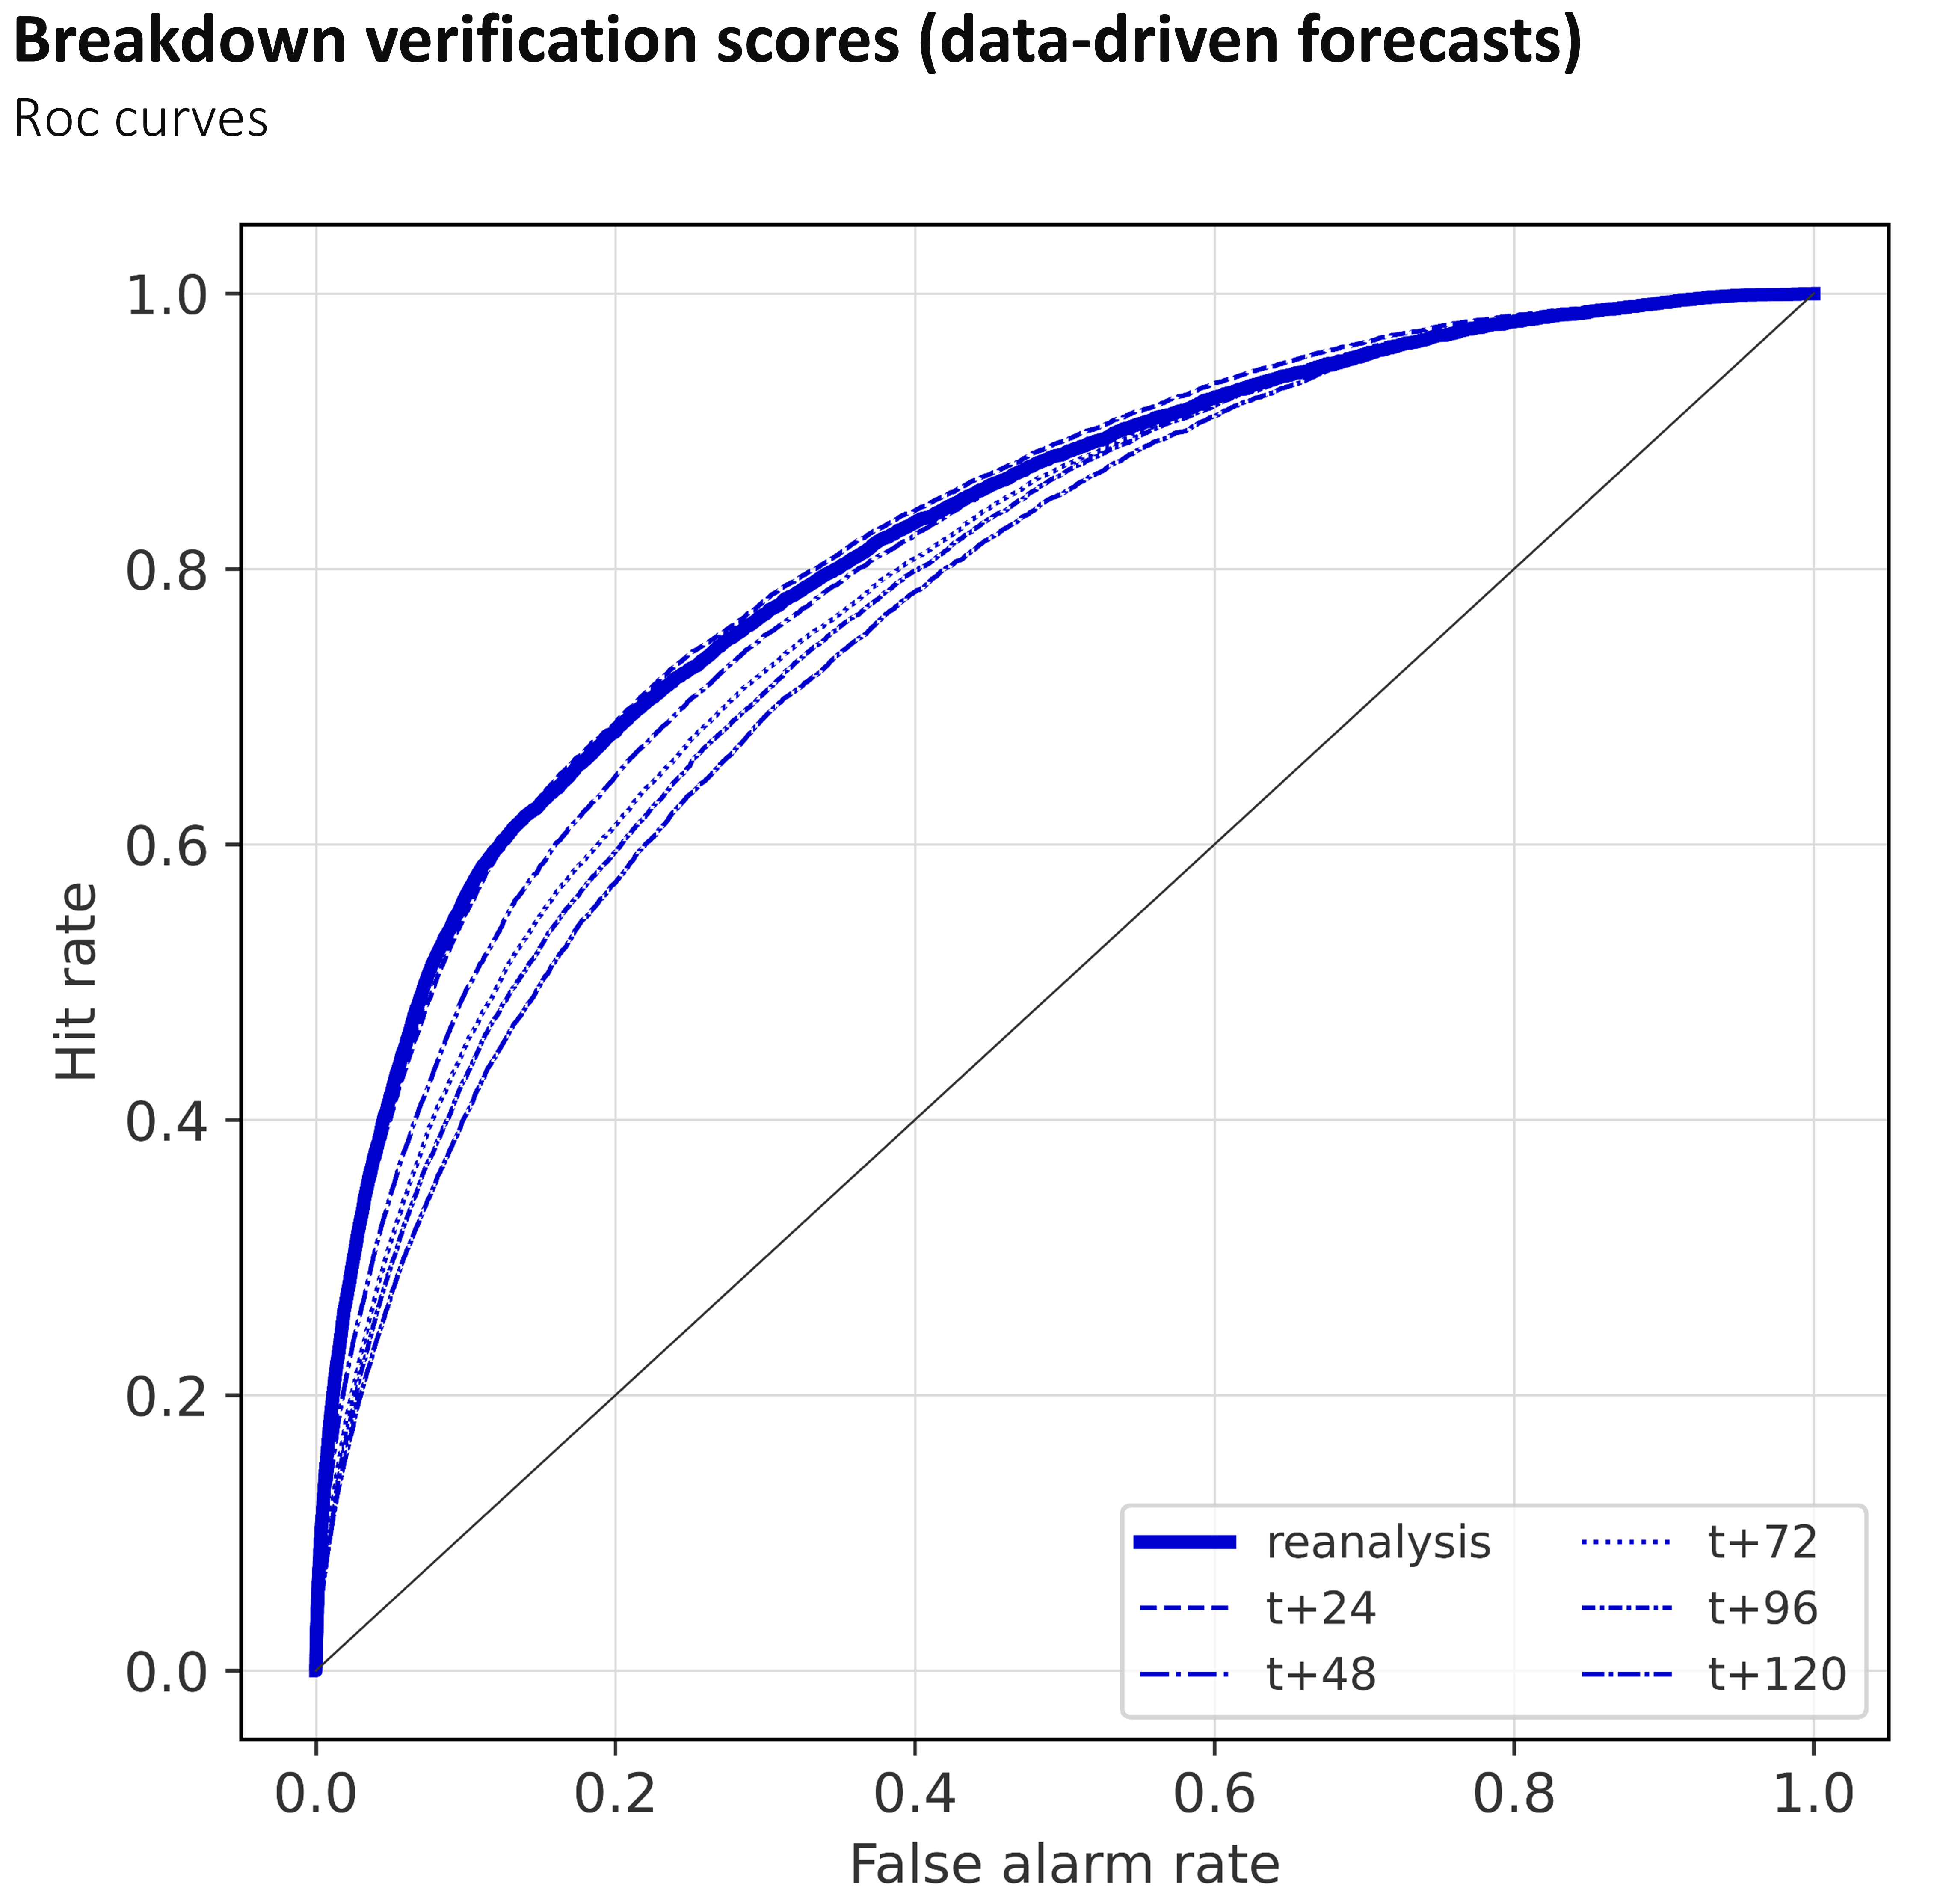
\includegraphics[width=\textwidth]{hydro_based_ff_verif_breakdown_scores_roc.png}
\caption{\textbf{Breakdown verification scores for data-driven, hydro-meteorological forecasts - ROC curves} Panels (a) to (f) show the ROC curves, respectively, for the short-range forecasts (i.e., reanalysis), for the long range forecasts at t+24 (day 1), t+48 (day 2), t+72 (day 3), t+96 (day 4), and t+120 (day 5).}
\label{fig:hydro_based_ff_verif_breakdown_scores_roc}
\end{figure}

From the reliability diagrams (Figure \ref{fig:hydro_based_ff_verif_breakdown_scores_rel_diag}) it is possible to understand better why the frequency bias increases significantly with the lead time \ref{fig:hydro_based_ff_verif_overall_scores}b. The reliability diagrams for day 0 (\ref{fig:hydro_based_ff_verif_breakdown_scores_rel_diag}a) and for day 1 (\ref{fig:hydro_based_ff_verif_breakdown_scores_rel_diag}b) are very similar. However, day 0 reliability shows a wider range of probabilities (up to \sim 15\%) with predicted probabilities similar to those observed than day 1 (with probabilities with this similar behaviour only up to \sim 10\%). At day 2 forecasts, the range of well calibrated probabilities diminishes up to 5\%, and from day 3, the predictions show mostly overestimation of the observed frequencies from forecasts probabilities exceeding 1\%. It is worth noticing how, also in the case of the rainfall-based forecasts, also the data-driven forecasts do not show a reduction of the issued probabilities with increasing lead times. As discussed in relevant section, this is due to the fact that we are using a rainfall forecasts that post-processed a deterministic system.

\begin{figure}[htbp]
\centering
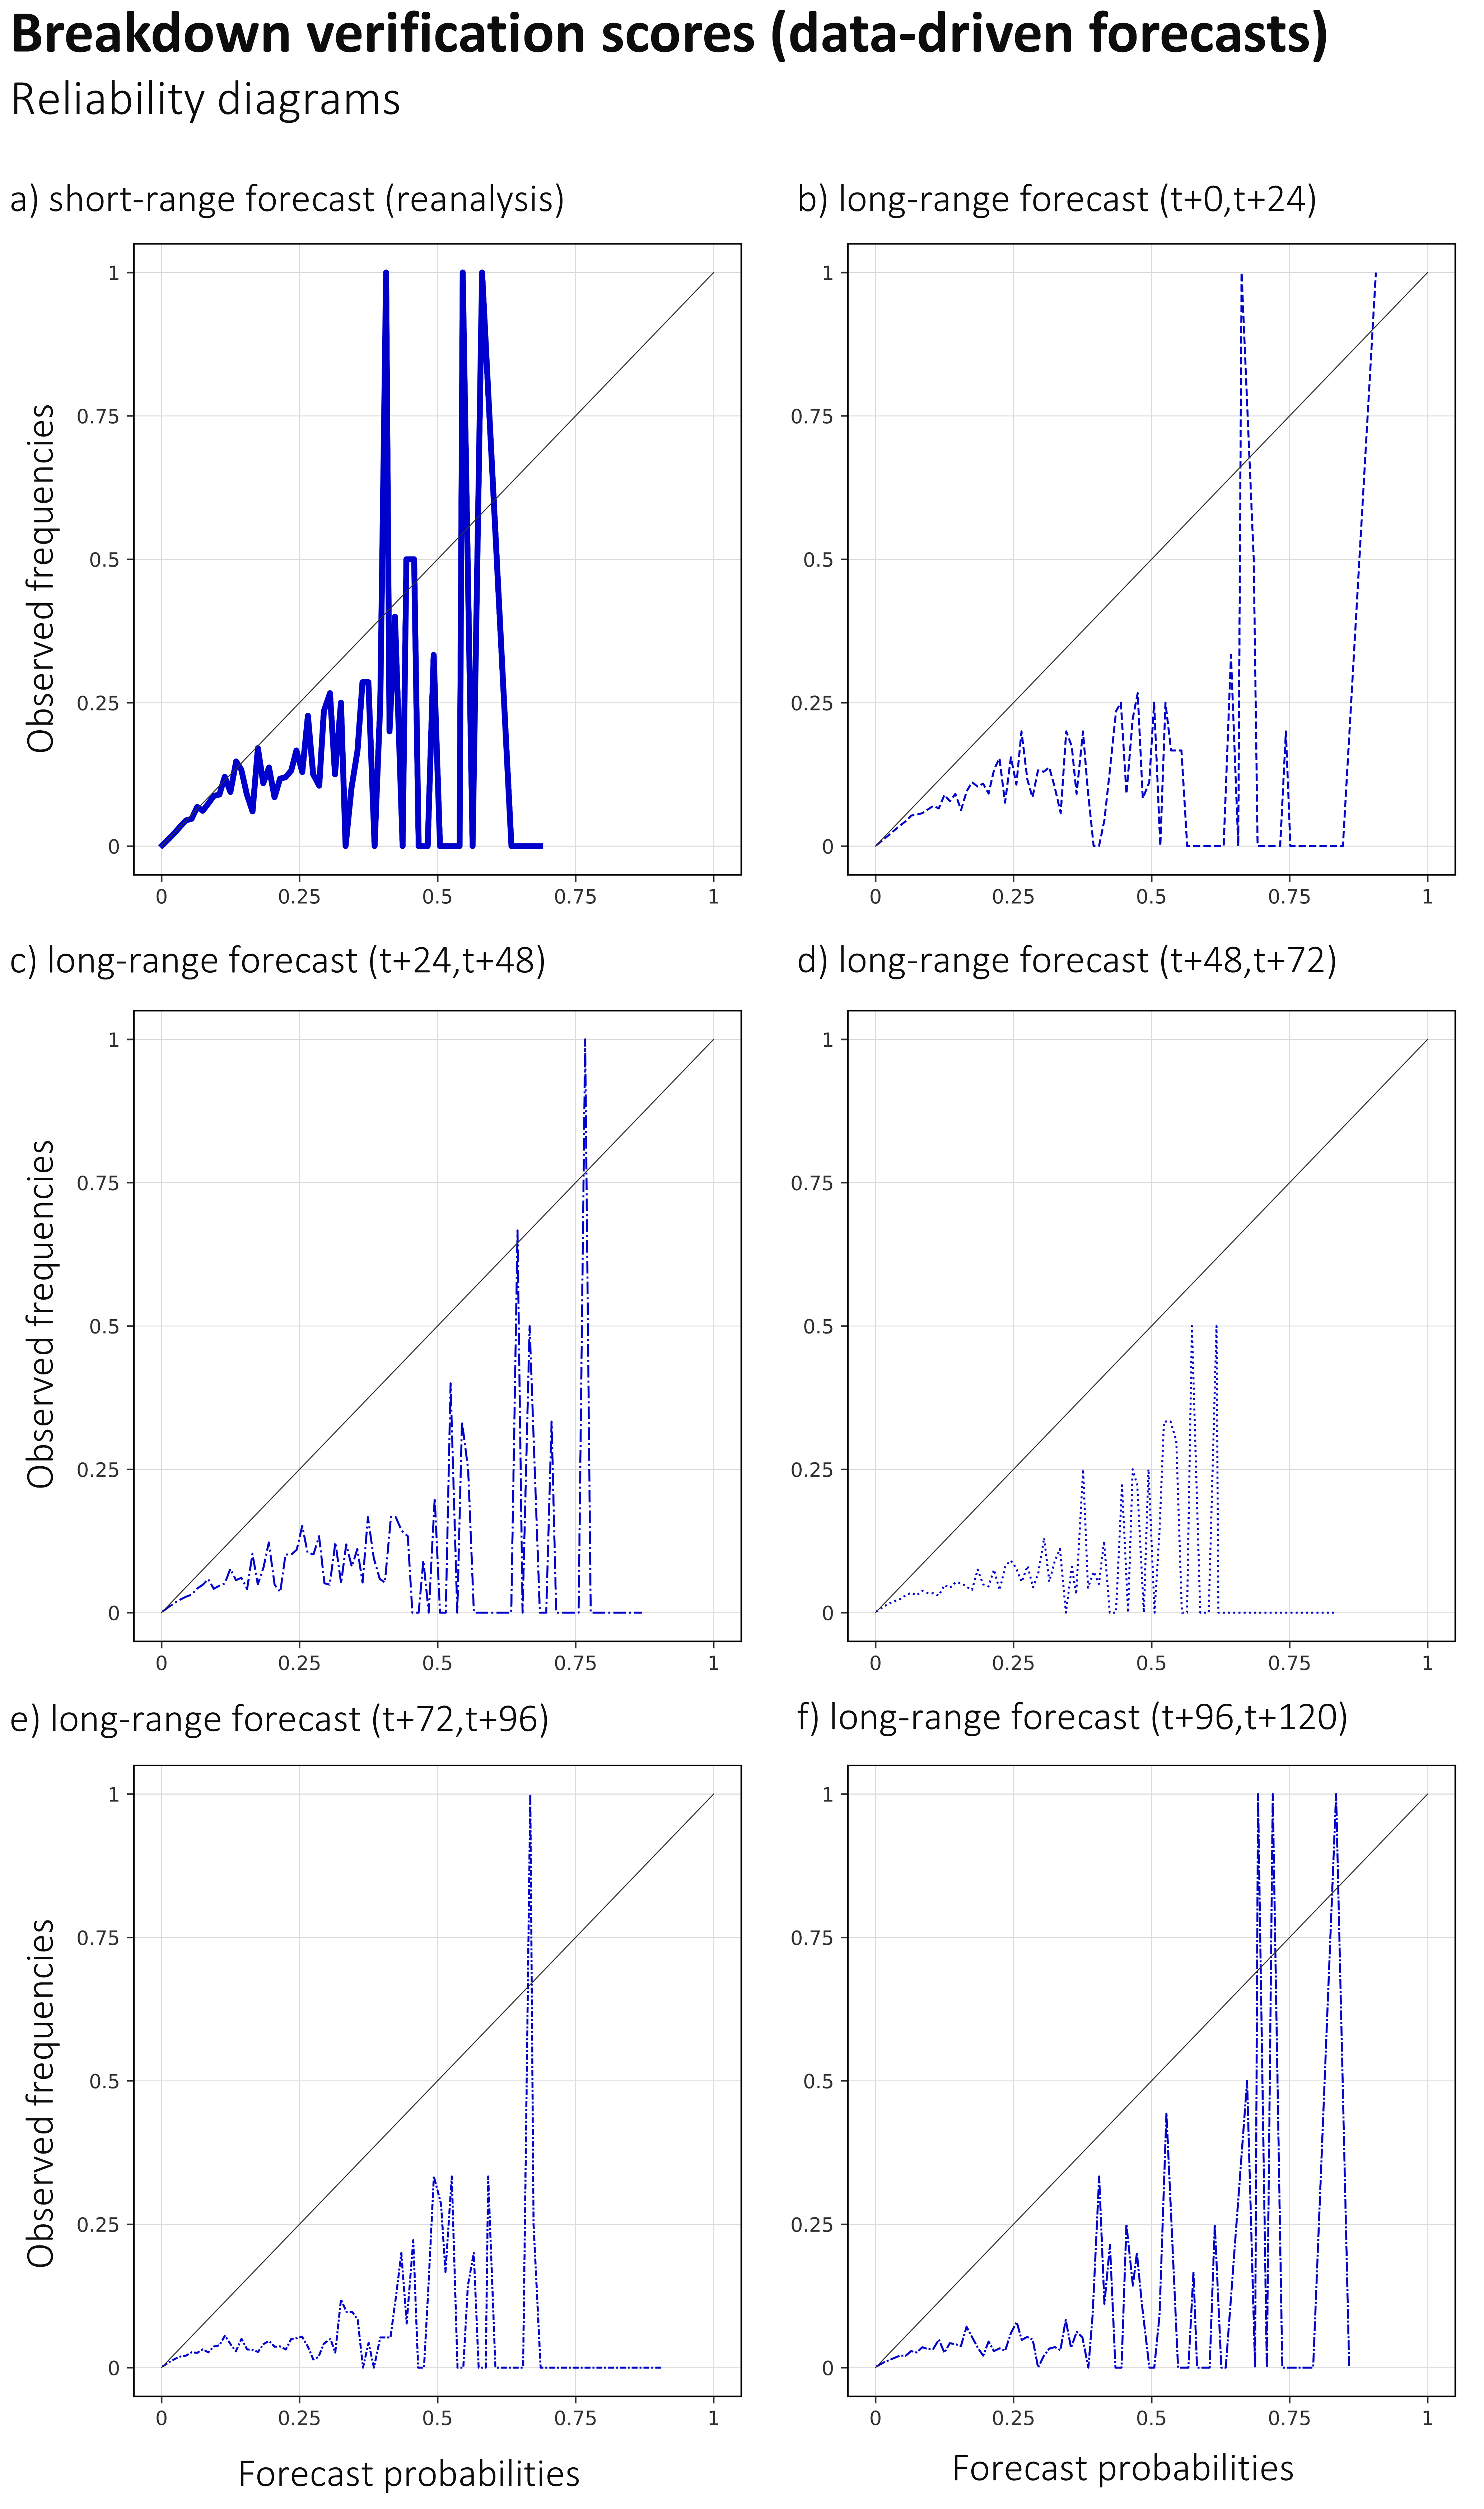
\includegraphics[width=\textwidth]{hydro_based_ff_verif_breakdown_scores_rel_diag.png}
\caption{\textbf{Breakdown verification scores for data-driven, hydro-meteorological forecasts - Reliability diagrams} Panels (a) to (f) show the reliability diagrams, respectively, for the short-range forecasts (i.e., reanalysis), for the long range forecasts at t+24 (day 1), t+48 (day 2), t+72 (day 3), t+96 (day 4), and t+120 (day 5).}
\label{fig:hydro_based_ff_verif_breakdown_scores_rel_diag}
\end{figure}


%%%%%%%%%%%%%%%%%%%%%%%%%%%%%%%%%%%%%%%%%%%%%%%%%%%%%%%%%%%%%%%%%%%%%%%
\subsection{Physical interpretation of the data-driven model behaviour}



%%%%%%%%%%%%%%%%%%%%%
\section{Discussions}
\label{data_driven_flash_floods_short_medium_range_discussions}

The results presented in the subsequent sections document the performance of both rainfall-based and data-driven hydro-meteorological forecasts. Section \ref{verif_rainfall_based_fc} shows the baseline verification results for the prediction of areas at risk of flash floods based using only ERA5-ecPoint short- and long-range rainfall predictions. Section \ref{verif_data_driven_short_fc} shows that the data-driven approach combining hydro-meteorological parameters yields statistically significant improvements in prediction skill, with particularly notable gains in discrimination ability as seen in the provided ROC curves. Section \ref{verif_data_driven_long_fc} shows that the predictive skill of the data-driven forecasts extends to day 5 with my better discrimination ability than its only rainfall-based counterpart. Section \ref{verif_case_study} shows a selection of flash flood events to illustrate the approaches' capacity to identify areas at risk of flash floods (in the US and around the world). Hence, the findings detailed in this chapter contribute to understanding how effectively current technologies can support flash flood warning systems.

%Optuna hyperparameter optimisation
% The random forest implementations show the least performance variations, while gradient boosting CatBoost, gradient Boosting LightGBM, and feed-forward neural network show the biggest variations. Reflecting enhanced minority class detection capabilities crucial for flash flood prediction. The consistency of optimal hyperparameter performance across different outer folds validates the robustness of the nested cross-validation framework.


%%%%%%%%%%%%%%%%%%%%%
\section{Conclusions}
\label{data_driven_flash_floods_short_medium_range_conclusions}

% Still to be completed.